%% 
%% Copyright 2019-2020 Elsevier Ltd
%% 
%% This file is part of the 'CAS Bundle'.
%% --------------------------------------
%% 
%% It may be distributed under the conditions of the LaTeX Project Public
%% License, either version 1.2 of this license or (at your option) any
%% later version.  The latest version of this license is in
%%    http://www.latex-project.org/lppl.txt
%% and version 1.2 or later is part of all distributions of LaTeX
%% version 1999/12/01 or later.
%% 
%% The list of all files belonging to the 'CAS Bundle' is
%% given in the file `manifest.txt'.
%% 
%% Template article for cas-sc documentclass for 
%% double column output.

%\documentclass[a4paper,fleqn,longmktitle]{cas-sc}
\documentclass[a4paper,fleqn]{cas-sc}

% \usepackage[numbers]{natbib}
%\usepackage[authoryear]{natbib}
\usepackage[authoryear,longnamesfirst]{natbib}

%%%Author definitions
\def\tsc#1{\csdef{#1}{\textsc{\lowercase{#1}}\xspace}}
\tsc{WGM}
\tsc{QE}
\tsc{EP}
\tsc{PMS}
\tsc{BEC}
\tsc{DE}
%%%

% Uncomment and use as if needed
%\newtheorem{theorem}{Theorem}
%\newtheorem{lemma}[theorem]{Lemma}
%\newdefinition{rmk}{Remark}
%\newproof{pf}{Proof}
%\newproof{pot}{Proof of Theorem \ref{thm}}

\usepackage[utf8]{inputenc}
%% for tables
\usepackage{booktabs}
\usepackage{siunitx}
\usepackage{threeparttable}
% \usepackage{tabularx}
% \usepackage{ragged2e}
\usepackage{rotating}
\usepackage{graphicx} 
\usepackage{geometry}
\usepackage{pdflscape} 
\usepackage{afterpage}
\usepackage{placeins}

%% new commands for better formatting
\newcommand{\sbf}[1]{\scriptsize\textbf{#1}}
\newcommand{\sit}[1]{\scriptsize\textit{#1}}
\newcommand{\dmidrule}{\specialrule{0.8pt}{0pt}{0.4pt}\specialrule{0.8pt}{0pt}{0pt}}
\usepackage{underscore}
\newcommand{\longvar}[1]{\textit{#1}}

\begin{document}
\let\WriteBookmarks\relax
\def\floatpagepagefraction{1}
\def\textpagefraction{.001}

% Short title
\shorttitle{Characterizing Ranking Environments}

% Short author
\shortauthors{}

% Main title of the paper
\title [mode = title]{Characterizing Ranking Environments: An Empirical Study of Technical and Content Attributes for System Profiling}                      
% Title footnote mark
% eg: \tnotemark[1]
\tnotemark[1,2]

% Title footnote 1.
% eg: \tnotetext[1]{Title footnote text}
% \tnotetext[<tnote number>]{<tnote text>} 
% \tnotetext[1]{This document is the results of the research
%    project funded by the National Science Foundation.}

% \tnotetext[2]{The second title footnote which is a longer text matter
%    to fill through the whole text width and overflow into
%    another line in the footnotes area of the first page.}


% % Corresponding author text
% \cortext[cor1]{Corresponding author}
% \cortext[cor2]{Principal corresponding author}

% Footnote text
% \fntext[fn1]{This is the first author footnote. but is common to third
%   author as well.}
% \fntext[fn2]{Another author footnote, this is a very long footnote and
%   it should be a really long footnote. But this footnote is not yet
%   sufficiently long enough to make two lines of footnote text.}

% % For a title note without a number/mark
% \nonumnote{This note has no numbers. In this work we demonstrate $a_b$
%   the formation Y\_1 of a new type of polariton on the interface
%   between a cuprous oxide slab and a polystyrene micro-sphere placed
%   on the slab.
%   }

% Here goes the abstract
\begin{abstract}
This study empirically characterized and compared Google's and Bing's ranking environments, analyzing technical performance (Lighthouse scores) and content attributes (lexical/semantic features) within a homogeneous commercial discount domain. Using \num{14465} SERP (Search Engine Results Page) items from 500 queries and 12 features, K-Means clustering identified six distinct web resource profiles, significantly associated with ranking tiers in both systems. Content-related attributes demonstrated a stronger aggregate association with visibility than technical scores for both Google (70.1\% importance) and Bing (61.8\%). Comparative analysis showed Bing's top-ranking results generally featured higher median values across numerous technical/content metrics than Google's. Notably for Google, high title-query semantic similarity unexpectedly associated with worse ranking odds in multivariate models, contrasting with positive main content-query similarity effects. Bing, conversely, prioritized content volume (word count) and explicit keyword signals more. These findings highlight system-specific nuances in factor weighting, contributing to IR system understanding and offering practical optimization insights. The dataset and analysis code will be made available upon publication.
\end{abstract}

% Use if graphical abstract is present
% \begin{graphicalabstract}
% \includegraphics{figs/grabs.pdf}
% \end{graphicalabstract}

% Research highlights
\begin{highlights}
\item Content factors show stronger aggregate link to SERP visibility than technical scores for Google (70.1\%) and Bing (61.8\%).
\item Google and Bing demonstrate significant differences in top-page attributes and inferred factor priorities.
\item Counterintuitive Google finding: High title-query semantic similarity linked to worse ranking (multivariate models).
\item Introduced a comparative profiling methodology for search engines using content-homogeneous data.
\end{highlights}

% Keywords
% Each keyword is seperated by \sep
\begin{keywords}
Ranking Factors \sep System Profiling \sep Technical Performance \sep Content Relevance \sep Semantic Similarity \sep Comparative Analysis
\end{keywords}


\maketitle

% --- INTRODUCTION ---
\section{Introduction}
\label{sec:intro}
\subsection{Background}
\label{subsec:background}
In contemporary digital society, large-scale information retrieval systems are primary gateways to vast online resources, fundamentally shaping how users discover and interact with information \citep{Coghlan2025}. Achieving visibility within these complex ranking environments is crucial for diverse online entities, from commercial enterprises to educational platforms \citep{Daly2024, Limongelli2022}. Ultimately, the success of these retrieval systems hinges on user satisfaction \citep{Wang2023}, a critical metric that reflects how well they meet diverse user needs and expectations. However, the algorithms governing visibility are notoriously complex and opaque, often described as "black boxes," making it challenging for resource creators and researchers to understand the precise factors driving organic ranking outcomes \citep{Coghlan2025, Roumeliotis2022}. This opacity also poses challenges for evaluating search engine effectiveness, particularly in specialized domains like e-commerce, where traditional metrics may not fully capture user experience, prompting calls for more user-oriented evaluation approaches \citep{Moffat2024}. Consequently, there is a growing interest in empirical approaches to infer the implicit priorities and behavioral patterns of these influential systems – a form of "reverse engineering" based on observational data.


\subsection{Problem Statement}
\label{subsec:problem}
A significant challenge in inferring system priorities is disentangling the influence of myriad factors. This is particularly true for the interplay between a resource's intrinsic content characteristics (e.g., relevance, quality, structure) and its technical performance attributes (e.g., loading speed, accessibility) \citep{Nagpal2021, Srinivas2025}. The sheer heterogeneity of content across the web often confounds attempts to isolate the specific impact of technical factors. Furthermore, while many studies investigate ranking factors within a single retrieval system (often implicitly Google) or focus on developing novel ranking algorithms to advance the state-of-the-art, large-scale comparative analyses characterizing the behavior of dominant, operational search engines remain relatively scarce. Such analyses are crucial for understanding how *different* major systems (e.g., Google vs. Bing) actually weigh various technical and content attributes in practice \citep{Toms2004}.

This study addresses this specific gap. It is an empirical investigation aimed at characterizing and profiling existing systems, rather than proposing a new ranking algorithm to outperform state-of-the-art models. It employed a methodological approach designed to mitigate content variance by analyzing a large dataset of online resources from a relatively homogenous domain – specifically, pages related to commercial discounts and promotional offers. This content similarity provided a controlled environment, allowing for better isolation of technical performance effects and exploration of potential system-specific preferences for content presentation or semantic relevance, thereby offering insights into the "black-box" nature of these widely-used information retrieval systems. Thus, the 'baselines' in this study refer to the existing operational search engines themselves, whose behaviors we aim to profile and compare.

\subsection{Research Objectives}
\label{subsec:aim}
This study aims to empirically characterize and compare the ranking environments of Google (System A) and Bing (System B) within a homogeneous domain. The specific research objectives designed to achieve this aim are:
\begin{enumerate}
\item To identify distinct profiles (clusters) of online resources based on a combination of their technical performance metrics (Lighthouse scores) and content characteristics (lexical and semantic features).
\item To determine if resources achieving higher SERP (Search Engine Results Page) visibility in Google and Bing are disproportionately associated with specific identified resource profiles.
\item To comparatively analyze the profiles and attribute distributions of top-ranking resources (e.g., top 5 positions) between Google and Bing for the same user queries.
\item To assess the relative strength of association between technical performance attributes versus content attributes and higher SERP visibility, comparing these patterns between Google and Bing.
\end{enumerate}

\subsection{Research Questions (RQs)}
\label{subsec:rqs}
This study sought to answer the following research questions:
\begin{itemize}
\item \textbf{RQ1 (Profiling \& Clustering of Online Resources):} Based on content relevance and Lighthouse metrics, what distinct profiles (clusters) emerged among the analyzed online resources? What were their defining characteristics?
\item \textbf{RQ2 (Ranking Patterns and Profile Associations):} Did resources ranking higher (e.g., top 5 vs. 6-20) in System A and System B tend to belong to specific profiles/clusters? How did the profiles of top-ranked resources differ from lower-ranked ones?
\item \textbf{RQ3 (System Differences):} How did the profiles of top-ranking resources differ between System A and System B for the same queries? Which content relevance or technical performance metrics appeared to be prioritized differently by these two retrieval systems within this domain?
\item \textbf{RQ4 (Technical vs. Content Weight):} Within the analyzed resource set, did technical performance metrics (measured by Lighthouse) or content relevance metrics show a stronger association with higher visibility rankings or specific 'successful' profiles? Did this differ between System A and System B?
\end{itemize}

\subsection{Contribution}
\label{subsec:contribution}
This research offers several contributions primarily focused on the empirical characterization of existing large-scale information retrieval systems, rather than the development of new state-of-the-art ranking algorithms. Methodologically, it presents a large-scale approach for comparative system profiling using a content-homogeneous dataset as a control variable to better isolate the effects of technical factors and content presentation strategies \citep{Jayaraman2022, Sezerrakolu2024}. Empirically, the study provides robust, data-driven insights into the apparent ranking behaviors of Google (System A) and Bing (System B) concerning key technical and content attributes within a commercially relevant domain. Theoretically and practically, the findings deepen the understanding of the differing operational logics of these major information retrieval systems, particularly highlighting counter-intuitive factor weightings under multivariate conditions, and offer potential insights for creators seeking to optimize resource visibility across different digital environments. The dataset and analysis scripts will be made available to foster reproducibility and enable further research by the community upon acceptance of the manuscript.

\subsection{Paper Structure}
\label{subsec:structure}
The remainder of this paper is organized as follows: Section \ref{sec:lit_review} reviews related work. Section \ref{sec:methodology} details the methodology. Section \ref{sec:results} presents the results. Section \ref{sec:discussion} discusses these findings. Section \ref{sec:data_code_availability} outlines the availability of the data and code. Finally, Section \ref{sec:conclusion} concludes the paper and suggests future research.
% --- END INTRODUCTION ---

% --- LITERATURE REVIEW ---
\section{Literature Review and Related Work}
\label{sec:lit_review}
\subsection{Factors Influencing Organic Visibility}
\label{subsec:lit_factors}

\subsubsection{Technical Performance and Resource Structure}
\label{subsubsec:lit_tech}
The technical underpinnings of online resources have long been recognized as crucial for visibility in retrieval systems. Beyond basic crawlability and indexability, factors like site speed, mobile-friendliness, security (HTTPS), and overall user experience related to performance are increasingly emphasized \citep{Roumeliotis2022}. This scope includes not only server-side performance and accessibility but also structural elements such as URL design. URL design can influence both user perception and machine interpretability for SEO \citep{Rastakhiz2024}. Retrieval systems also invest heavily in identifying and penalizing manipulative or low-quality content. This task shares challenges with areas like phishing detection, where hybrid feature models are employed for robustness \citep{Zhu2024}. Tools like Google's Lighthouse provide standardized metrics for performance, accessibility, adherence to best practices, and basic technical SEO checks. These metrics offer quantifiable indicators of technical health. Furthermore, concepts derived from link analysis, such as PageRank, remain foundational in understanding resource authority and trustworthiness \citep{Srinivas2025, Toms2004}. Ongoing research continues to develop sophisticated models to assess website trust and combat misinformation \citep{Niu2022}.

\subsubsection{Content Signals and Semantic Relevance}
\label{subsubsec:lit_content}
While technical aspects form the foundation, content remains a primary driver of relevance. Early approaches focused heavily on keyword matching and density \citep{Srinivas2025}. Modern retrieval systems, however, employ sophisticated Natural Language Processing (NLP) techniques moving beyond lexical matching towards semantic understanding \citep{Jindal2014}. This is crucial as users are often driven by a desire to reduce uncertainty or engage with interesting content \citep{vanderSluis2025}, motivations that are better served by semantically rich and relevant results rather than mere keyword presence. Techniques like Latent Semantic Analysis (LSA) \citep{Nagpal2021}, topic modeling, and more recently, vector embeddings from deep learning models like Sentence-BERT, allow for capturing semantic similarity even without exact keyword overlap \citep{Pauzi2023}. Understanding user intent and matching it with semantically relevant content is paramount \citep{Jindal2014, Limongelli2022}.

\subsubsection{Measuring Content Quality and User Experience Signals}
\label{subsubsec:lit_quality}
Defining and measuring "content quality" is inherently complex. Beyond relevance, factors such as readability, structure, originality, depth, and authority contribute to quality perceptions. Linguistic frameworks, like applying Grice's conversational maxims, offer structured ways to evaluate content clarity, informativeness, and appropriateness \citep{Sezerrakolu2024}. Retrieval systems may also incorporate implicit user feedback signals (e.g., click-through rates, dwell time) as proxies for content quality and user satisfaction. However, these signals are harder for external researchers to measure directly.

\subsubsection{Synthesizing Technical and Content Factors}
\label{subsubsec:lit_synthesis}
Understanding the interplay between technical performance and content quality/relevance is crucial. Some studies suggest a trade-off or differing importance depending on context. Examples include the stage of the user journey \citep{Nagpal2021} or the specific retrieval system being analyzed \citep{Toms2004}. Modeling approaches sometimes attempt to integrate these diverse factors to predict ranking outcomes or system behavior \citep{Jayaraman2022}. The relative weighting assigned by different systems remains an active area of investigation.

\subsection{Profiling and Characterizing Online Resources}
\label{subsec:lit_profiling}
Given the diversity of online resources, methods for grouping or classifying them based on shared characteristics are valuable. Clustering algorithms (e.g., K-Means, Hierarchical) can identify emergent profiles. These profiles are based on quantitative features like performance scores or content metrics \citep{Yu2024}. Content analysis, including automated dictionary-based methods, can classify resources based on their topical focus or expressed attributes \citep{Milei2025}. Such profiling helps in an understanding the different strategies or archetypes present within a specific domain or result set.

\subsection{Comparative Analysis of Information Retrieval Systems}
\label{subsec:lit_comparison}
While Google (System A) dominates market share, Bing (System B) and others represent significant alternative access points to information. Comparing their ranking behaviors is important for a comprehensive understanding of the information ecosystem. Studies have historically noted differences in how systems weigh factors like link structure versus content \citep{Toms2004}. Understanding these differences is crucial for creators aiming for broad visibility. Furthermore, ethical considerations and potential biases embedded within the ranking logic of different systems are increasingly important topics \citep{Coghlan2025}.

\subsection{Reverse Engineering Approaches in Information Retrieval}
\label{subsec:lit_reverse}
Due to the proprietary nature of commercial ranking algorithms, researchers often resort to "black-box" analysis or reverse engineering. This involves systematically correlating observable input features (resource attributes) with observable output behavior (rankings). The goal is to infer potential algorithmic priorities. While unable to reveal exact algorithms, such empirical studies can provide valuable insights. They highlight factors strongly associated with higher visibility within specific system environments \citep{Bardas2025}. Modern approaches increasingly explore sophisticated optimization objectives beyond simple relevance. One example is incorporating risk-sensitivity into deep learning ranking models to improve the robustness and fairness of outcomes \citep{SilvaRodrigues2025}.

\subsection{Research Gap}
\label{subsec:lit_gap}
Despite extensive research on individual ranking factors and retrieval systems, a gap exists. **For instance, while key comparative studies like \citet{Toms2004} identified differing system priorities, they often operated on heterogeneous datasets where variations in content type could confound the results. It thus remains challenging to isolate whether observed ranking differences stem from fundamental algorithmic philosophies or from the systems' varied responses to different content genres.** This study aims to fill this gap by not only characterizing and contrasting the ranking environments of System A and System B within a specific commercial context but also by employing a methodology that combines modern technical audits (Lighthouse) with advanced semantic feature analysis (Sentence-BERT) on a content-homogeneous dataset to reveal nuanced factor prioritizations and system-specific profiles. This can better isolate technical effects and system-specific content preferences in comparative system profiling.
% --- END LITERATURE REVIEW ---

% --- METHODOLOGY ---
\section{Methodology}
\label{sec:methodology}
This section details the systematic approach undertaken to collect, process, and prepare the data. The goal was to characterize and compare the ranking environments of two major information retrieval systems.

\subsection{Research Design}
\label{subsec:design}
This study employed a quantitative, observational research design. Data pertaining to resource visibility (rankings) and associated attributes (technical performance, content features) were collected programmatically from Google (System A) and Bing (System B). Subsequent analysis involved data mining and statistical techniques to profile resources and infer system priorities.

\subsection{Data Collection}
\label{subsec:collection}
Data collection occurred around April 17, 2025.
\subsubsection{Query Set Preparation}
\label{subsubsec:queries}
The query set comprised 500 unique English search queries. These queries focused on online commercial promotions and discounts. They were curated to balance broad coverage with reduced semantic redundancy (e.g., '[Brand] promo code'). The full list is available in the accompanying dataset (\texttt{keywords.csv}). The dataset will be made publicly available upon acceptance of the manuscript. This domain homogeneity was a methodological choice to control for content variance.

\subsubsection{Retrieval System Data Acquisition}
\label{subsubsec:serp_acq}
For each query, the top $\sim$20 organic results were retrieved from Google (via Google Custom Search API) and Bing (via Bing Web Search API). Default API settings were used to minimize personalization. Raw JSON responses (URLs, titles, snippets, rank positions) were saved.

\subsubsection{Resource Content Acquisition}
\label{subsubsec:content_acq}
Unique URLs were visited using a headless browser (Puppeteer via \texttt{pyppeteer}). This process saved full HTML content and captured screenshots. Access/rendering errors were logged.

\subsection{Feature Engineering}
\label{subsec:features}
\subsubsection{Main Content Extraction}
\label{subsubsec:trafilatura}
The \texttt{trafilatura} library \citep{Barbaresi2021} extracted the main textual content from saved HTML, excluding boilerplate.

\subsubsection{Technical Performance Features (Lighthouse)}
\label{subsubsec:lighthouse}
The Google PageSpeed Insights API provided four core Lighthouse scores (Performance, Accessibility, Best Practices, SEO) for each URL \citep{Roumeliotis2022}.

\subsubsection{Content Relevance and Attribute Features}
\label{subsubsec:content_features}
Eight content features were extracted for each query-URL pair:
\begin{enumerate}
\item \textbf{Lexical Features:} $query\_in\_title$ (all query words in HTML title), \longvar{exact_query_in_title} (exact query string in title), $query\_in\_h1$ (all query words in first \texttt{<h1>}), $exact\_query\_in\_h1$ (exact query string in first \texttt{<h1>}), $query\_density\_body$ (percentage of query string in main text), and $word\_count$ (alphabetic words in main text).
\item \textbf{Semantic Similarity Features:} Using Sentence-BERT ('all-mpnet-base-v2' \citep{Reimers2019, Song2020}), cosine similarity was calculated for $semantic\_similarity\_title\_query$ (query vs. HTML title) and \longvar{semantic_similarity_content_query} (query vs. main text). Long texts for the latter were chunked \citep{Beltagy2020, Devlin2019}.
\end{enumerate}
All feature extraction was performed using custom Python scripts. These scripts leveraged libraries such as BeautifulSoup for HTML parsing, NLTK for tokenization, and Trafilatura for main content extraction. The analysis scripts will be made publicly available upon acceptance of the manuscript.

\subsection{Dataset Description and Preprocessing}
\label{subsec:assembly}
This study utilizes a custom-compiled dataset specifically designed for the empirical characterization and comparison of the ranking environments of Google (System A) and Bing (System B). To ensure a controlled analytical environment by mitigating content variance, the dataset exclusively comprises web resources from a homogeneous domain: online commercial promotions and discount offers (as detailed in Section \ref{subsubsec:queries}).

The data collection pipeline, which involved querying for 500 unique English keywords (focused on said domain) across both search engines, initially yielded approximately \num{19950} raw SERP results. Following the programmatic acquisition of webpage content, comprehensive feature engineering (see Section \ref{subsec:features} for details on the 12 technical and content features extracted), and necessary data cleaning and filtering (e.g., exclusion of $\sim$1.25\% of entries with missing Lighthouse data), the \textbf{final dataset for analysis comprises \num{14465} individual SERP result items}. Each item in this dataset represents a unique query-URL pair, annotated with its organic search rank position and the suite of extracted features. The structure of these entries and feature descriptions are detailed in Table \ref{tab:dataset_columns_types}.

The dataset encompasses \textbf{\num{6929} unique URLs} from \textbf{\num{2238} unique hostnames}. The distribution of SERP items is \num{5895} for Google and \num{8570} for Bing. It is pertinent to note that the $pwa\_score$ Lighthouse feature was entirely removed from the feature set due to 100\% missing values across all collected data points.

Descriptive statistics for all numerical features in the final dataset, including an outlier analysis, are presented in Table \ref{tab:comprehensive_stats}. While some features exhibited outliers (e.g., $performance\_score$: 5.45\%; $exact\_query\_in\_title$: 16.63\%; $query\_density\_body$: 12.09\%), these were generally retained to reflect real-world data variability. Robust statistical methods were employed in subsequent analyses where appropriate to account for these distributions. For multivariate analyses, including K-Means clustering and Ordinal Logistic Regression, all numerical features were Min-Max scaled to a [0,1] range to ensure equitable feature contribution and improve model performance.


\begin{table}[htbp!]
\centering
\begin{threeparttable}
\caption{Dataset Column Types and Descriptions}
\label{tab:dataset_columns_types}
\small
\setlength{\tabcolsep}{3pt}
\renewcommand{\arraystretch}{1}
\begin{tabular*}{\textwidth}{l@{\extracolsep{\fill}}lll}
\toprule
\sbf{Category} & \sbf{Column Name} & \sbf{Type} & \sbf{Description (Metric)} \\
\dmidrule
Search Engine & engine & Categorical (google/bing) & Search Engine \\
Search Engine & position & Integer (1-20) & SERP Position \\
\midrule
Lighthouse & performance\_score & Float (0-100) & Perf. \\
Lighthouse & accessibility\_score & Float (0-100) & Access. \\
Lighthouse & best-practices\_score & Float (0-100) & Best Prac. \\
Lighthouse & seo\_score & Float (0-100) & SEO \\
\midrule
Content & query\_in\_title & Integer (0/1) & Q-Title \\
Content & query\_in\_h1 & Integer (0/1) & Q-H1 \\
Content & exact\_query\_in\_title & Integer (0/1) & ExQ-Title \\
Content & exact\_query\_in\_h1 & Integer (0/1) & ExQ-H1 \\
Content & query\_density\_body & Float (\%) & Q/B Density \\
Content & semantic\_similarity\_title\_query & Float (0-1, Cosine) & Sim. Title \\
Content & semantic\_similarity\_content\_query & Float (0-1, Cosine) & Sim. Content \\
Content & word\_count & Integer & Word Count \\
\bottomrule
\end{tabular*}
\begin{tablenotes}[flushleft]
\scriptsize
\item Metric abbreviations: Perf. (Performance Score), Access. (Accessibility Score), Best Prac. (Best Practices Score), SEO (SEO Score), Q-Title (Query in Title), Q-H1 (Query in H1), ExQ-Title (Exact Query in Title), ExQ-H1 (Exact Query in H1), Q/B Density (Query Density Body), Sim. Title (Semantic Similarity Title-Query), Sim. Content (Semantic Similarity Content-Query).
\end{tablenotes}
\end{threeparttable}
\end{table}


\begin{table}[htbp!]
\centering
\begin{threeparttable}
\caption{Descriptive Statistics of the Final Analyzed Dataset (N=\num{14465})}
\label{tab:comprehensive_stats}
\small
\setlength{\tabcolsep}{3pt}
\renewcommand{\arraystretch}{1}
\begin{tabular*}{\textwidth}{l@{\extracolsep{\fill}}S[table-format=3.2]S[table-format=3.2]S[table-format=4.2]S[table-format=3.2]S[table-format=6.2]S[table-format=3.2]S[table-format=3.2]S[table-format=2.2]}
\toprule
\sbf{Metric} & \sbf{Mean} & \sbf{Median} & \sbf{SD} & \sbf{Min} & \sbf{Max} & \sbf{Q1} & \sbf{Q3} & \sbf{IQR\%} \\
\dmidrule
\multicolumn{9}{l}{\sit{SERP Position}} \\
Overall & 10.15 & 10.00 & 5.67 & 1.00 & 20.00 & 5.00 & 15.00 & 0.00 \\
\midrule
\multicolumn{9}{l}{\sit{Lighthouse Scores}} \\
Perf. & 87.83 & 95.00 & 15.04 & 12.00 & 100.00 & 82.00 & 99.00 & 5.45 \\
Access. & 87.36 & 90.00 & 8.45 & 34.00 & 100.00 & 83.00 & 94.00 & 2.96 \\
Best Prac. & 91.75 & 96.00 & 12.09 & 37.00 & 100.00 & 85.00 & 100.00 & 4.14 \\
SEO & 93.00 & 92.00 & 7.43 & 40.00 & 100.00 & 92.00 & 100.00 & 3.21 \\
\midrule
\multicolumn{9}{l}{\sit{Content Relevance Metrics}} \\
Q-Title & 0.41 & 0.00 & 0.49 & 0.00 & 1.00 & 0.00 & 1.00 & 0.00 \\
Q-H1 & 0.38 & 0.00 & 0.49 & 0.00 & 1.00 & 0.00 & 1.00 & 0.00 \\
ExQ-Title & 0.17 & 0.00 & 0.37 & 0.00 & 1.00 & 0.00 & 0.00 & 16.63 \\
ExQ-H1 & 0.15 & 0.00 & 0.36 & 0.00 & 1.00 & 0.00 & 0.00 & 14.88 \\
Q/B Density & 0.19 & 0.00 & 0.46 & 0.00 & 7.73 & 0.00 & 0.20 & 12.09 \\
Sim. Title & 0.68 & 0.76 & 0.22 & -0.02 & 1.00 & 0.65 & 0.81 & 12.22 \\
Sim. Content & 0.58 & 0.62 & 0.18 & -0.04 & 0.88 & 0.49 & 0.72 & 2.24 \\
Word Count & 628.56 & 428.00 & 1294.32 & 0.00 & 132115.00 & 168.00 & 795.00 & 6.24 \\
\bottomrule
\end{tabular*}
\begin{tablenotes}[flushleft]
\scriptsize
\item Note: SD = Standard Deviation; Q1 = First Quartile; Q3 = Third Quartile. IQR\% indicates percentage of outliers via IQR method.
\item Metric abbreviations are defined in Table \ref{tab:dataset_columns_types}.
\end{tablenotes}
\end{threeparttable}
\end{table}






\subsection{Data Analysis Strategy}
\label{subsec:analysis_strategy}
The preprocessed dataset was analyzed using Python (v3.9+). Key libraries included Pandas, NumPy, Scikit-learn, Statsmodels, and SciPy. The significance level $\alpha$ was set to $0.05$. Numerical features were Min-Max scaled to [0,1] for multivariate analyses.

\subsubsection{RQ1: Resource Profiling and Clustering}
\label{subsubsec:analysis_rq1}
K-Means clustering was applied to 12 scaled technical and content features. The optimal number of clusters, $K=6$, was determined using the Elbow method and Silhouette analysis (Figure \ref{fig:rq1_optimal_clusters}). Clusters were characterized by their mean feature values (Table \ref{tab:rq1_cluster_summary}; Figure \ref{fig:rq1_cluster_radar_normalized}). Kruskal-Wallis H-tests (Table \ref{app:rq1_cluster_validation_table}) and Random Forest Classifier feature importances identified discriminative features.

\subsubsection{RQ2: Visibility Patterns versus Profiles}
\label{subsubsec:analysis_rq2}
Resources were grouped into High (1-5), Medium (6-10), and Low (11-20) rank tiers for Google and Bing separately.
\begin{itemize}
\item \textbf{Profile Distribution:} Pearson's $\chi^2$ test assessed the association between profiles and rank tiers.
\item \textbf{Feature Comparison:} Kruskal-Wallis H-test (with Dunn's post-hoc) compared median feature values across rank tiers (Table \ref{tab:rq2_kruskal_wallis_ranks}).
\end{itemize}

\subsubsection{RQ3: Comparative System Analysis (Google vs. Bing)}
\label{subsubsec:analysis_rq3}
Top-ranking (1-5) resources were compared between Google and Bing.
\begin{itemize}
\item \textbf{Profile Comparison:} Pearson's $\chi^2$ test compared profile distributions.
\item \textbf{Feature Comparison:} Mann-Whitney U test compared median feature values. Cohen's $d$ estimated the effect size.
\end{itemize}

\subsubsection{RQ4: Inferring Factor Priorities (Technical vs. Content)}
\label{subsubsec:analysis_rq4}
Several methods were used:
\begin{itemize}
\item \textbf{Correlation Analysis:} Spearman's $\rho$ correlated features with SERP $position$.
\item \textbf{Ordinal Logistic Regression:} A Proportional Odds Logit model (`statsmodels.miscmodels.ordinal\_model.OrderedModel`) predicted SERP quintiles (0=best to 4=worst). This was done using technical-only, content-only, and combined scaled feature sets. Model fit (Pseudo $R^2$, AIC, BIC) and coefficient significance/direction were examined \citep{Nagpal2021, Toms2004}. A negative coefficient indicated a higher probability of a better rank. (Full models are in \ref{app:rq4_regression_tables}). \\
The validity of all reported ordinal logistic regression models (technical-only, content-only, and combined) was confirmed by testing the proportional odds assumption. In all cases, the assumption was met (e.g., Brant test p>.05), supporting the robustness of the reported coefficients across ranking quintiles.
\item \textbf{Random Forest Feature Importance:} A Regressor predicted numerical SERP position. This was used to derive Gini importance for features, aggregated for technical versus content factors.
\end{itemize}
Non-parametric tests were used where parametric assumptions were violated.
% --- END METHODOLOGY ---

% --- RESULTS ---
\section{Results}
\label{sec:results}
This section presents empirical findings from the dataset analysis.

\subsection{RQ1: Derived Resource Profiles}
\label{subsec:results_rq1}
K-Means clustering on 12 scaled features identified six distinct resource profiles. The optimal $K=6$ (Silhouette score: \num{0.442}) is shown in Figure \ref{fig:rq1_optimal_clusters}. All features differed significantly across clusters (Kruskal-Wallis, $p < .001$; Table \ref{app:rq1_cluster_validation_table}). The internal cohesion and separation quality of these six profiles were quantitatively assessed using Silhouette and Calinski-Harabasz scores, as presented in Table \ref{tab:cluster_quality}. These metrics provide a global and per-cluster evaluation of the clustering solution's robustness. As the table indicates, while the overall structure is reasonable (Average Silhouette Score: 0.442), the quality varies across profiles, with Cluster 2 showing the highest internal cohesion.


To better understand the structure of the clusters and their interrelationships, the results of a Principal Component Analysis (PCA) on the 12 features are visualized in Figure \ref{fig:pca_visualization}. These first two components explain 43.0\% of the total variance in the dataset. An analysis of the PCA loadings reveals that the First Principal Component (PC1) represents a strategic trade-off between Comprehensive Content \& Technical Health (negative values) and Direct Keyword Targeting (positive values). The Second Principal Component (PC2) reflects a similar balance between Exact-Match Keyword Targeting (negative values) and Overall Technical Performance (positive values). Specifically, PC1 was most strongly driven by high positive loadings from \texttt{query\_in\_title} and \texttt{semantic\_similarity\_title\_query}, and high negative loadings from \texttt{word\_count} and \texttt{accessibility\_score}. Meanwhile, PC2 primarily contrasted Overall Technical Performance (positive loading from \texttt{performance\_score}) against Exact-Match Keyword Targeting (negative loading from \texttt{exact\_query\_in\_h1}).

On this strategic map, the positions of the clusters corroborate the profiles presented in Table \ref{tab:rq1_cluster_summary}. For instance, Cluster 3 (orange), located on the far left of the PC1 axis, represents resources with high word counts but weak keyword targeting, while Cluster 4 (pink), concentrated on the right, indicates a profile that adopts aggressive keyword optimization. The notable overlap observed between clusters suggests that many web resources employ hybrid strategies, a finding that is consistent with the moderate average Silhouette score of 0.442.


Mean scaled feature values for each cluster are in Table \ref{tab:rq1_cluster_summary} and visualized in Figure \ref{fig:rq1_cluster_radar_normalized}.
Key profiles include:
\begin{itemize}
\item \textbf{Cluster 2 ("High Keyword \& Semantic Relevance, Strong Technicals"; 16.3\%):} Excelled across most metrics.
\item \textbf{Cluster 3 ("Low Relevance, Low Technicals"; 16.0\%):} Performed poorly (e.g., $semantic\_similarity\_title\_query$ mean scaled: \num{0.269}; $word\_count$ median: \num{61}).
\end{itemize}
Other clusters (0, 1, 4, 5) showed varied specializations. $Query\_in\_title$, $query\_in\_h1$, and $semantic\_similarity\_title\_query$ were most influential in cluster differentiation.

\begin{figure}[htbp!]
    \centering
    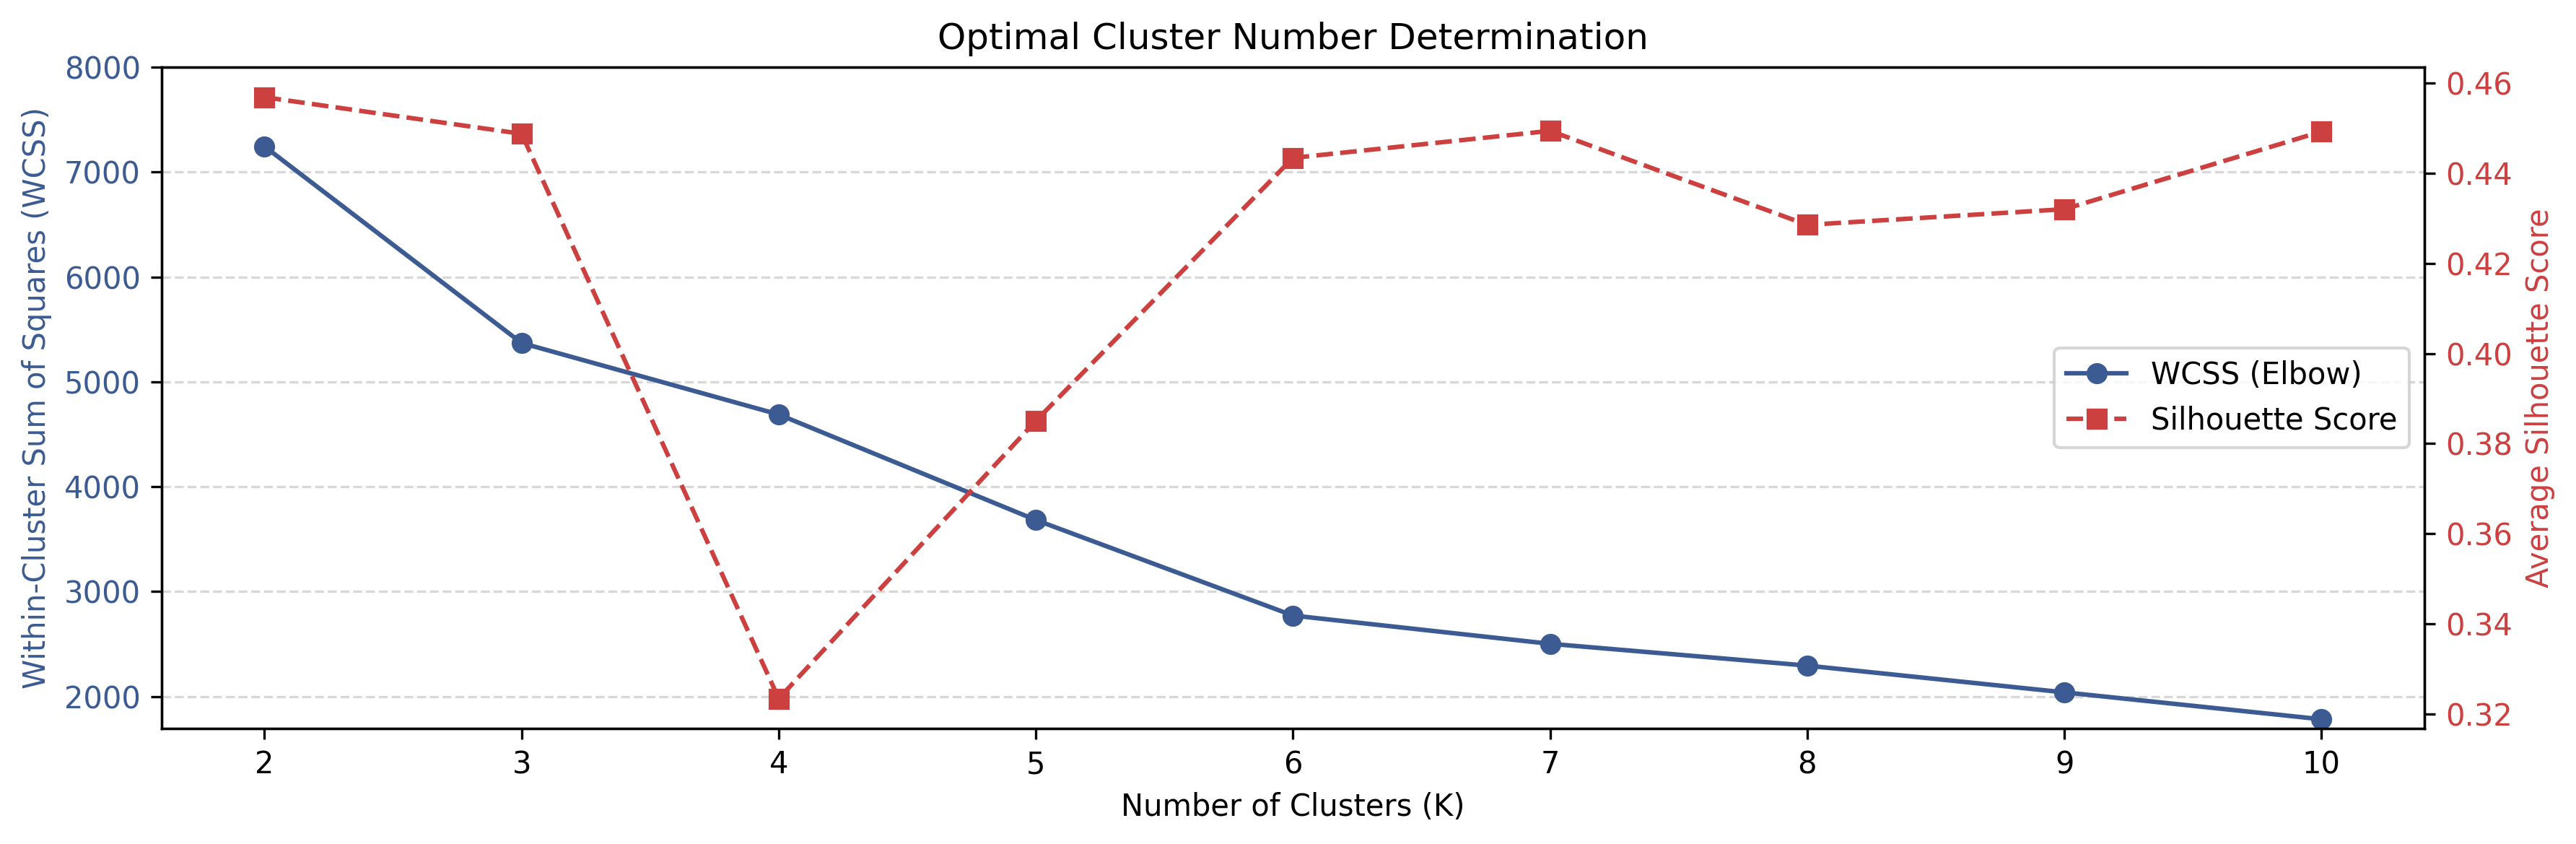
\includegraphics[width=1\linewidth]{figs/rq1_optimal_clusters_combined.png}
    \caption{Determination of optimal cluster number ($K$) using Elbow method (left Y-axis, WCSS) and Silhouette analysis (right Y-axis, Average Silhouette Score). $K=6$ was selected.}
    \label{fig:rq1_optimal_clusters}
\end{figure}

\begin{table}[htbp!]
\centering
\caption{Mean Scaled Feature Values for the Six Identified Cluster Profiles (RQ1)}
\label{tab:rq1_cluster_summary}
\small 
\setlength{\tabcolsep}{3pt}
\renewcommand{\arraystretch}{1}
\begin{tabular*}{\textwidth}{l@{\extracolsep{\fill}} S[table-format=1.3] S[table-format=1.3] S[table-format=1.3] S[table-format=1.3] S[table-format=1.3] S[table-format=1.3] }
\toprule
\sbf{Feature (Scaled)} & {{\sbf{C0}}} & {{\sbf{C1}}} & {{\sbf{C2}}} & {{\sbf{C3}}} & {{\sbf{C4}}} & {{\sbf{C5}}} \\
\dmidrule
Perf. & 0.858 & 0.870 & 0.881 & 0.811 & 0.870 & 0.871 \\
Access. & 0.806 & 0.823 & 0.826 & 0.736 & 0.805 & 0.837 \\
Best Prac. & 0.853 & 0.879 & 0.880 & 0.826 & 0.899 & 0.866 \\
SEO & 0.880 & 0.897 & 0.906 & 0.776 & 0.911 & 0.921 \\
Q-Title & 0.000 & 0.000 & 1.000 & 0.000 & 1.000 & 1.000 \\
Q-H1 & 1.000 & 0.000 & 1.000 & 0.000 & 0.000 & 1.000 \\
ExQ-Title & 0.000 & 0.000 & 1.000 & 0.000 & 0.187 & 0.000 \\
ExQ-H1 & 0.166 & 0.000 & 0.818 & 0.000 & 0.000 & 0.105 \\
Q/B Density & 0.031 & 0.010 & 0.072 & 0.000 & 0.046 & 0.016 \\
Sim. Title & 0.759 & 0.729 & 0.823 & 0.269 & 0.790 & 0.778 \\
Sim. Content & 0.747 & 0.716 & 0.758 & 0.389 & 0.711 & 0.730 \\
Word Count & 0.005 & 0.005 & 0.006 & 0.003 & 0.003 & 0.005 \\
\midrule
Cluster Size (N) & {1054} & {5142} & {2122} & {2314} & {1522} & {2311} \\
Percentage (\%) & {7.3} & {35.5} & {14.7} & {16.0} & {10.5} & {16.0} \\
\bottomrule
\end{tabular*}
\begin{tablenotes}[flushleft]
\scriptsize
\item Note: C0-C5 represent Cluster 0 to Cluster 5. Features were Min-Max scaled to [0,1].
\item Metric abbreviations are defined in Table \ref{tab:dataset_columns_types}.
\end{tablenotes}
\end{table}


\begin{table}[htbp!]
\centering
\caption{Identified Cluster Quality and Cohesion Metrics (RQ1)}
\label{tab:cluster_quality}
\small
\setlength{\tabcolsep}{3pt}
\renewcommand{\arraystretch}{1}
\begin{threeparttable}
\begin{tabular*}{\textwidth}{l@{\extracolsep{\fill}} S[table-format=4.0] S[table-format=2.1] S[table-format=1.3] S[table-format=6.1]}
\toprule
\sbf{Cluster Profile} & {\sbf{Cluster Size (N)}} & {\sbf{Percentage (\%)}} & {\sbf{Mean Silhouette Score}} & {\sbf{WCSS}} \\
\dmidrule
C0: Balanced Profile & 1054 & 7.3 & 0.493 & 484.8 \\
C1: Low Relevance & 5142 & 35.5 & 0.451 & 532.5 \\
C2: Content Focused & 2122 & 14.7 & 0.544 & 439.2 \\
C3: Low Relevance \& Poor Technicals & 2314 & 16.0 & 0.222 & 569.7 \\
C4: High Relevance & 1522 & 10.5 & 0.444 & 485.6 \\
C5: Technical Excellence & 2311 & 16.0 & 0.521 & 252.9 \\
\midrule
\sbf{Overall / Average} & \sbf{14465} & \sbf{100.0} & \sbf{0.442} & \sbf{2764.5} \\
\bottomrule
\end{tabular*}
\begin{tablenotes}[flushleft]
\scriptsize
\item Note: Higher Silhouette scores indicate better-defined clusters. Lower WCSS indicates tighter clusters. Cluster sizes are from Table \ref{tab:rq1_cluster_summary}.
\end{tablenotes}
\end{threeparttable}
\end{table}


\begin{table}[htbp!]
\centering
\caption{Kruskal-Wallis H-Test Results for Feature Differentiation Across Clusters (RQ1)}
\label{app:rq1_cluster_validation_table}
\small
\setlength{\tabcolsep}{3pt}
\renewcommand{\arraystretch}{1}
\begin{threeparttable}
\begin{tabular*}{\textwidth}{l@{\extracolsep{\fill}} S[table-format=5.3] S[table-format=1.3,table-comparator=true]}
\toprule
\sbf{Feature} & {\sbf{H-statistic}} & {\sbf{p-value}} \\
\dmidrule
Perf.  & 232.613 & < .001 \\
Access.  & 920.863 & < .001 \\
Best Prac.  & 171.951 & < .001 \\
SEO  & 1756.283 & < .001 \\
Q-Title  & 14464.000 & < .001 \\
Q-H1  & 14464.000 & < .001 \\
ExQ-Title  & 12798.195 & < .001 \\
ExQ-H1  & 9102.510 & < .001 \\
Q/B Density  & 4388.283 & < .001 \\
Sim. Title  & 7561.791 & < .001 \\
Sim. Content  & 4641.727 & < .001 \\
Word Count  & 2015.283 & < .001 \\
\bottomrule
\end{tabular*}
\begin{tablenotes}[flushleft]
\scriptsize
\item All p-values reported as $< .001$ were originally $0.0$ in the source data.
\item Metric abbreviations are defined in Table \ref{tab:dataset_columns_types}.
\end{tablenotes}
\end{threeparttable}
\end{table}


\begin{figure}[htbp!]
 \centering
    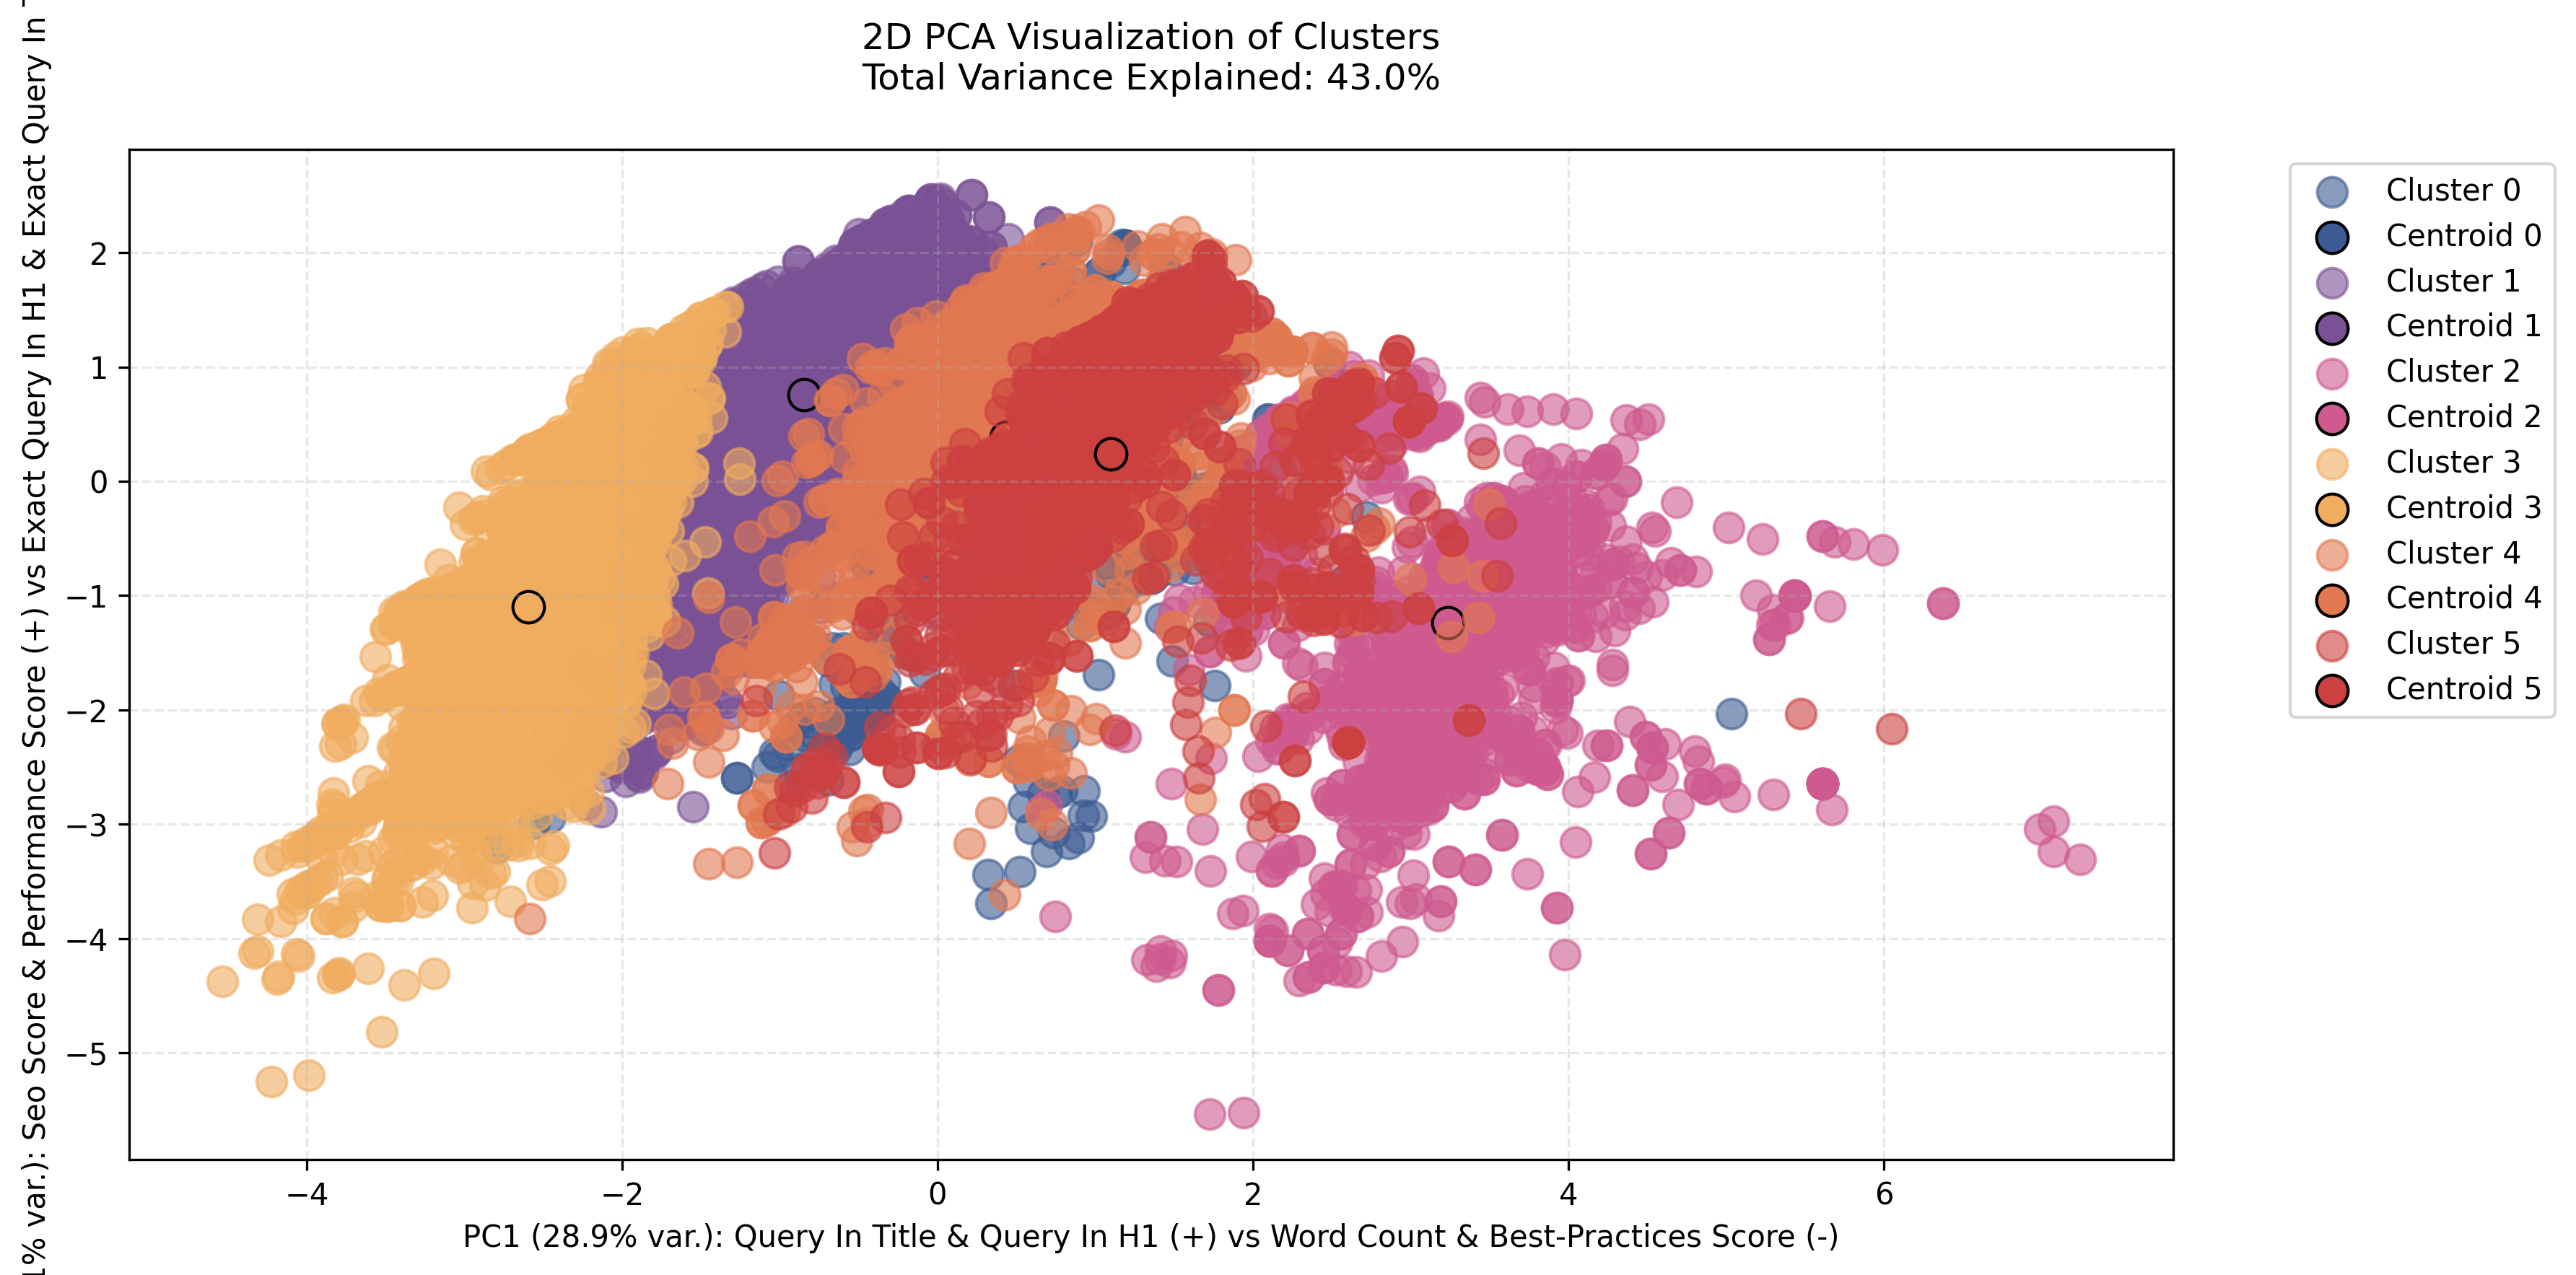
\includegraphics[width=\columnwidth]{figs/rq1_cluster_pca_2d.png}
    \caption{2D PCA visualization of the six identified cluster profiles. 
    The first component (PC1) contrasts direct keyword targeting against 
    content volume and technical health, while the second component (PC2) 
    contrasts overall technical performance against exact-match keyword targeting.}
    \label{fig:pca_visualization}
\end{figure}

\begin{figure}[htbp!]
    \centering
    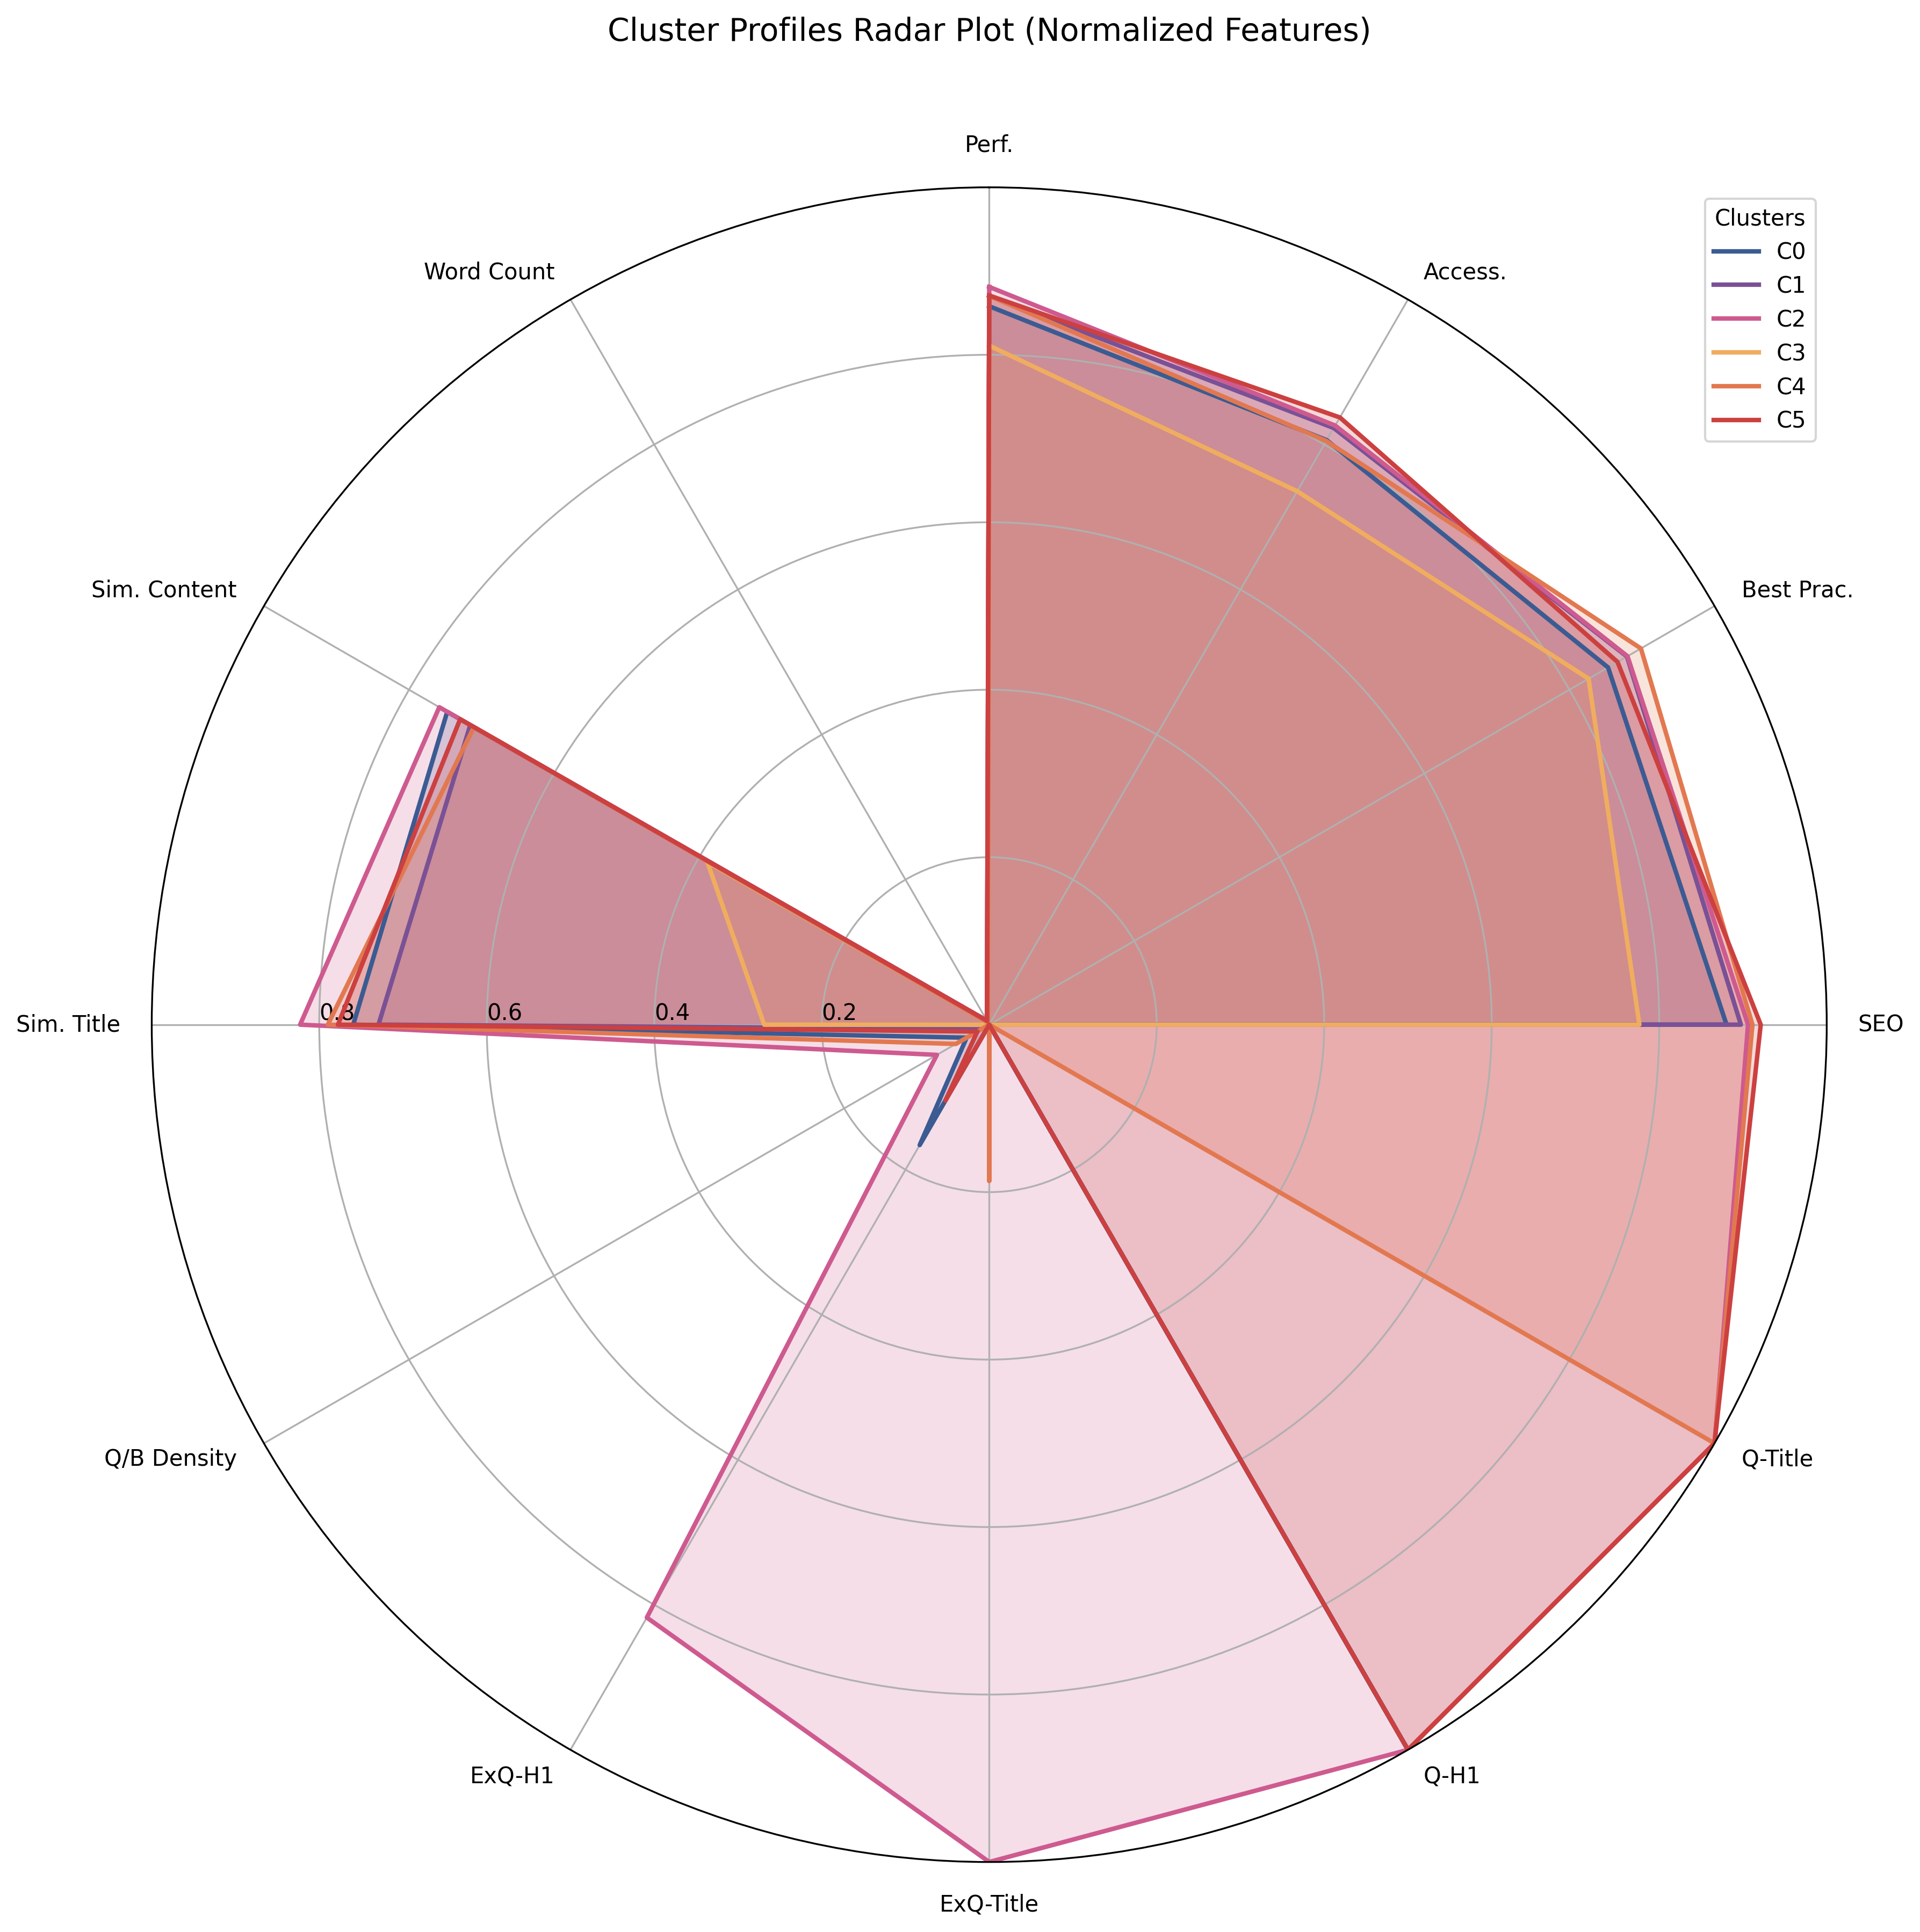
\includegraphics[width=1\linewidth]{figs/rq1_cluster_radar_normalized.png}
    \caption{Radar plot of mean scaled feature values for the six cluster profiles (RQ1).}
    \label{fig:rq1_cluster_radar_normalized}
\end{figure}

\subsection{RQ2: Visibility Patterns and Profiles}
\label{subsec:results_rq2}
\textbf{Profile Distribution across Ranks:} A significant association was found between cluster membership and ranking tiers for both engines (Pearson's $\chi^2, p < .001$; Figure \ref{fig:rq2_profile_dist_combined}). For Google, Profile 3 ("Low Relevance, Low Technicals") was more prevalent in lower ranks. For Bing, Profiles 1 and 2 were more prominent in higher ranks.

\begin{figure}[htbp!]
    \centering
    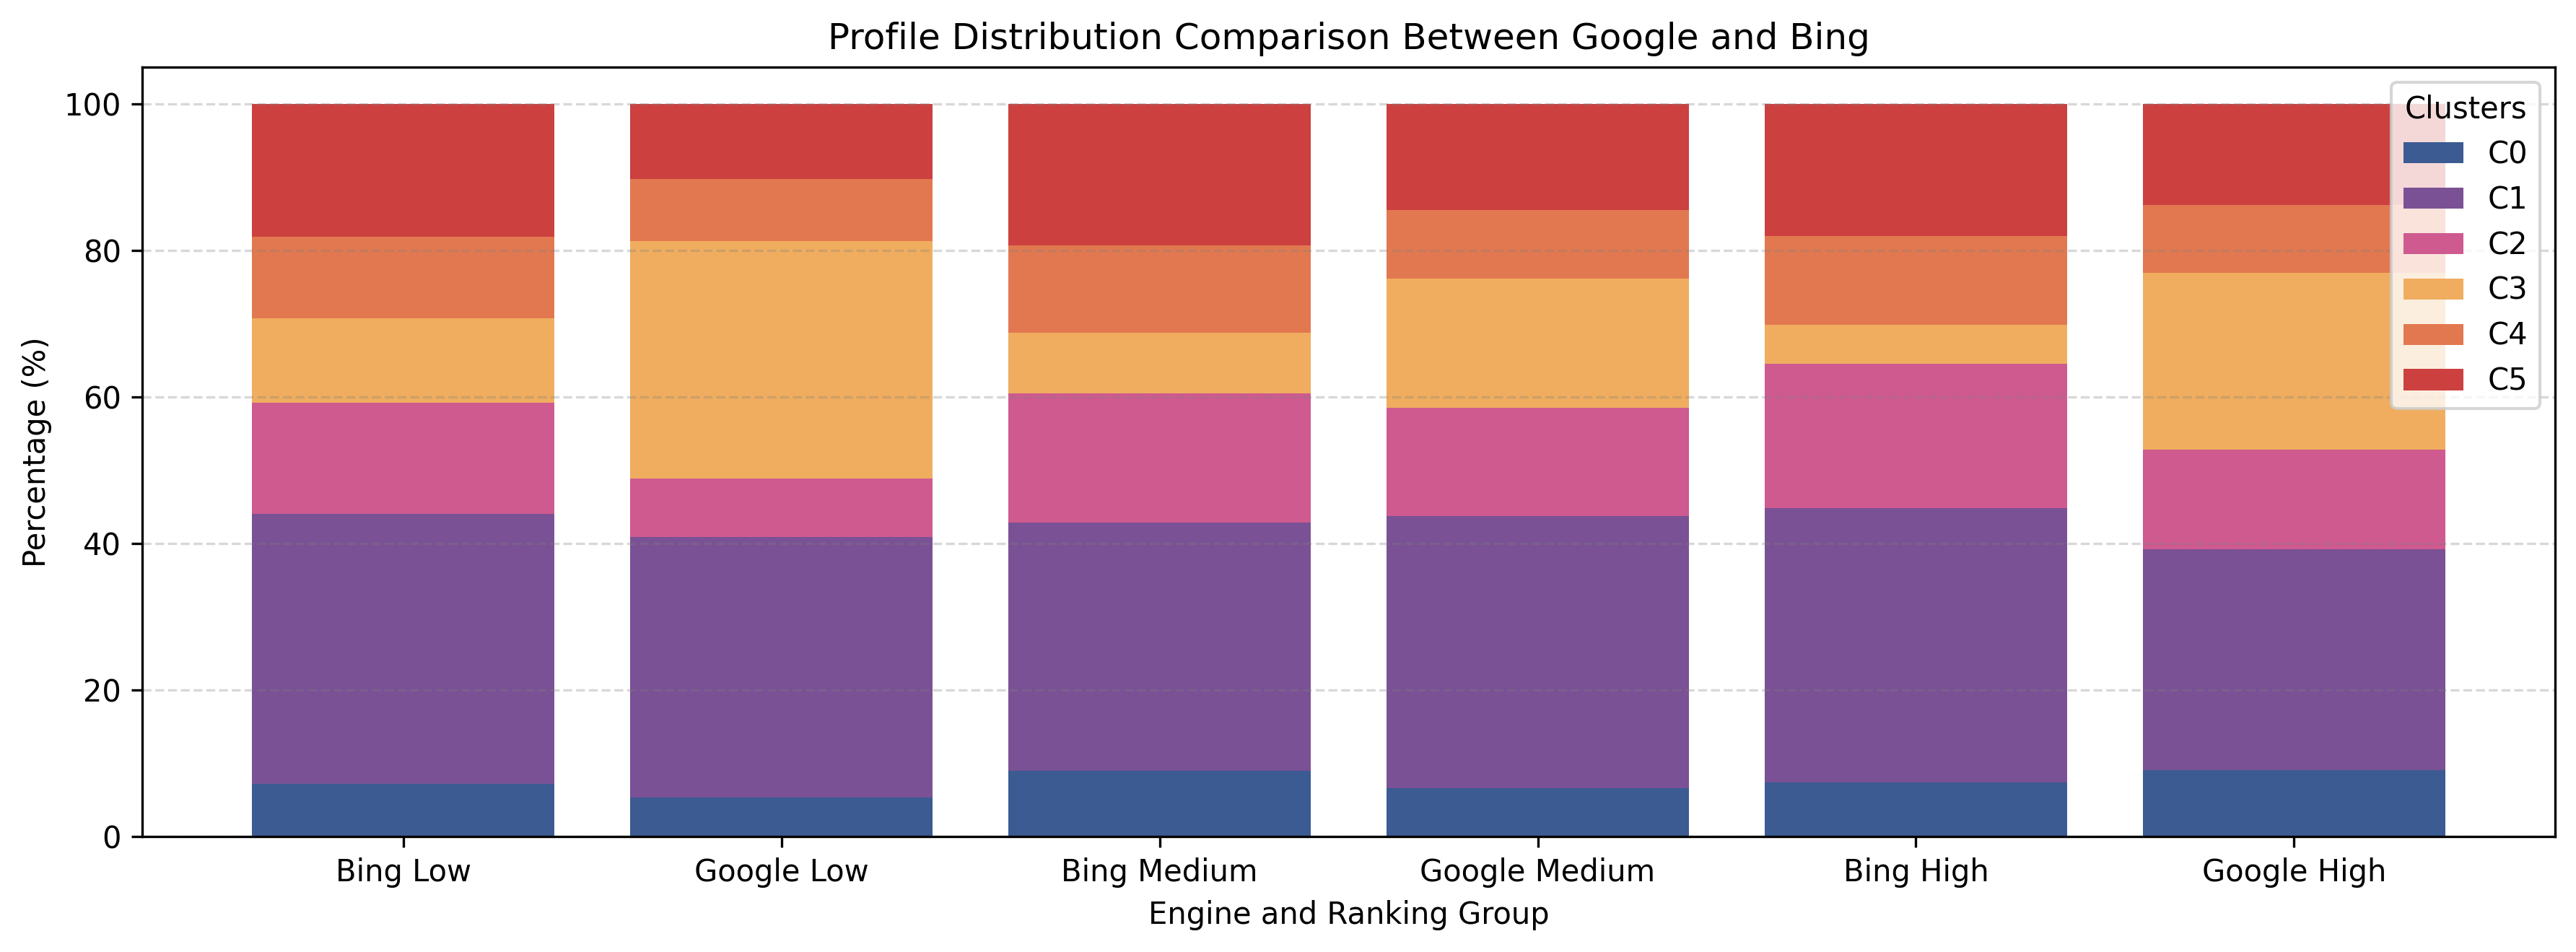
\includegraphics[width=1\linewidth]{figs/rq2_profile_dist_combined_grouped_bar.png}
    \caption{Profile Distribution Across Ranking Groups for Google and Bing (RQ2).}
    \label{fig:rq2_profile_dist_combined}
\end{figure}

\textbf{Feature Comparison across Ranks:} Kruskal-Wallis H-tests (Table \ref{tab:rq2_kruskal_wallis_ranks}) indicated significant differences ($p < .05$) for all Lighthouse scores and most content metrics across ranking groups for both systems.
\begin{itemize}
\item For Google, higher median $semantic\_similarity\_content\_query$ (High: 0.606) and $accessibility\_score$ (High: 91.0) were associated with better ranks.
\item For Bing, $accessibility\_score$ (High: 91.0), $semantic\_similarity\_title\_query$ (High: 0.785), and $word\_count$ (High: 630) showed clearer positive associations with better ranking tiers.
\end{itemize}

% Table for RQ2 Kruskal-Wallis Results
\begin{table}[htbp!]
\centering
\caption{Kruskal-Wallis H-Test Results for Features Across Ranking Tiers (High, Medium, Low) for Google and Bing (RQ2)}
\label{tab:rq2_kruskal_wallis_ranks}
\small
\setlength{\tabcolsep}{3pt}
\renewcommand{\arraystretch}{1}
\begin{threeparttable}
\begin{tabular*}{\textwidth}{l@{\extracolsep{\fill}}S[table-format=3.3] S[table-format=1.3,table-comparator=true] S[table-format=3.3] S[table-format=1.3,table-comparator=true]}
\toprule
& \multicolumn{2}{c}{\sbf{Google (System A)}} & \multicolumn{2}{c}{\sbf{Bing (System B)}} \\
\cmidrule(lr){2-3} \cmidrule(lr){4-5}
\sbf{Feature} & {\sbf{H-statistic}} & {\sbf{p-value}} & {\sbf{H-statistic}} & {\sbf{p-value}} \\
\dmidrule
\sit{Lighthouse Scores} & & & & \\
Perf. & 35.896 & < .001 & 86.829 & < .001 \\
Access. & 29.247 & < .001 & 359.950 & < .001 \\
Best Prac. & 27.224 & < .001 & 1.773 & 0.412 \\
SEO & 102.804 & < .001 & 32.794 & < .001 \\
\midrule
\sit{Content Relevance Metrics} & & & & \\
Q-Title & 79.726 & < .001 & 21.592 & < .001 \\
Q-H1 & 109.376 & < .001 & 23.123 & < .001 \\
ExQ-Title & 45.916 & < .001 & 12.440 & 0.002 \\
ExQ-H1 & 43.171 & < .001 & 33.618 & < .001 \\
Q/B Density & 91.336 & < .001 & 127.544 & < .001 \\
Sim. Title & 207.318 & < .001 & 89.876 & < .001 \\
Sim. Content & 242.241 & < .001 & 9.394 & 0.009 \\
Word Count & 30.762 & < .001 & 595.954 & < .001 \\
\bottomrule
\end{tabular*}
\begin{tablenotes}[flushleft]
\scriptsize
\item Ranking Tiers: High (1-5), Medium (6-10), Low (11-20).
\item Dunn's test for post-hoc comparisons not shown here.
\item Metric abbreviations are defined in Table \ref{tab:dataset_columns_types}.
\end{tablenotes}
\end{threeparttable}
\end{table}



\subsection{RQ3: Comparative System Analysis (Google vs. Bing)}
\label{subsec:results_rq3}
\textbf{Profile Comparison in Top Ranks:} A significant difference ($\chi^2(5) \approx 302.26, p < .001$) was found in profile distribution within the top 5 ranks (Figure \ref{fig:rq3_profile_comparison}). While Cluster 1 was the most common profile in Bing's top 5, Google's top results, though also led by Cluster 1 (Low Relevance), 
featured a significantly larger proportion of profiles like Cluster 3 (Low Relevance \& Poor Technicals) and Cluster 4 (High Relevance).

\textbf{Feature Comparison in Top Ranks:} Bing's top-ranking pages generally had significantly higher median scores for most features (Mann-Whitney U, $p < .005$; Table \ref{tab:rq3_feature_comparison}). These included $semantic\_similarity\_title\_query$ (medium effect size) and $word\_count$ (small effect size).

\begin{figure}[htbp!]
\centering
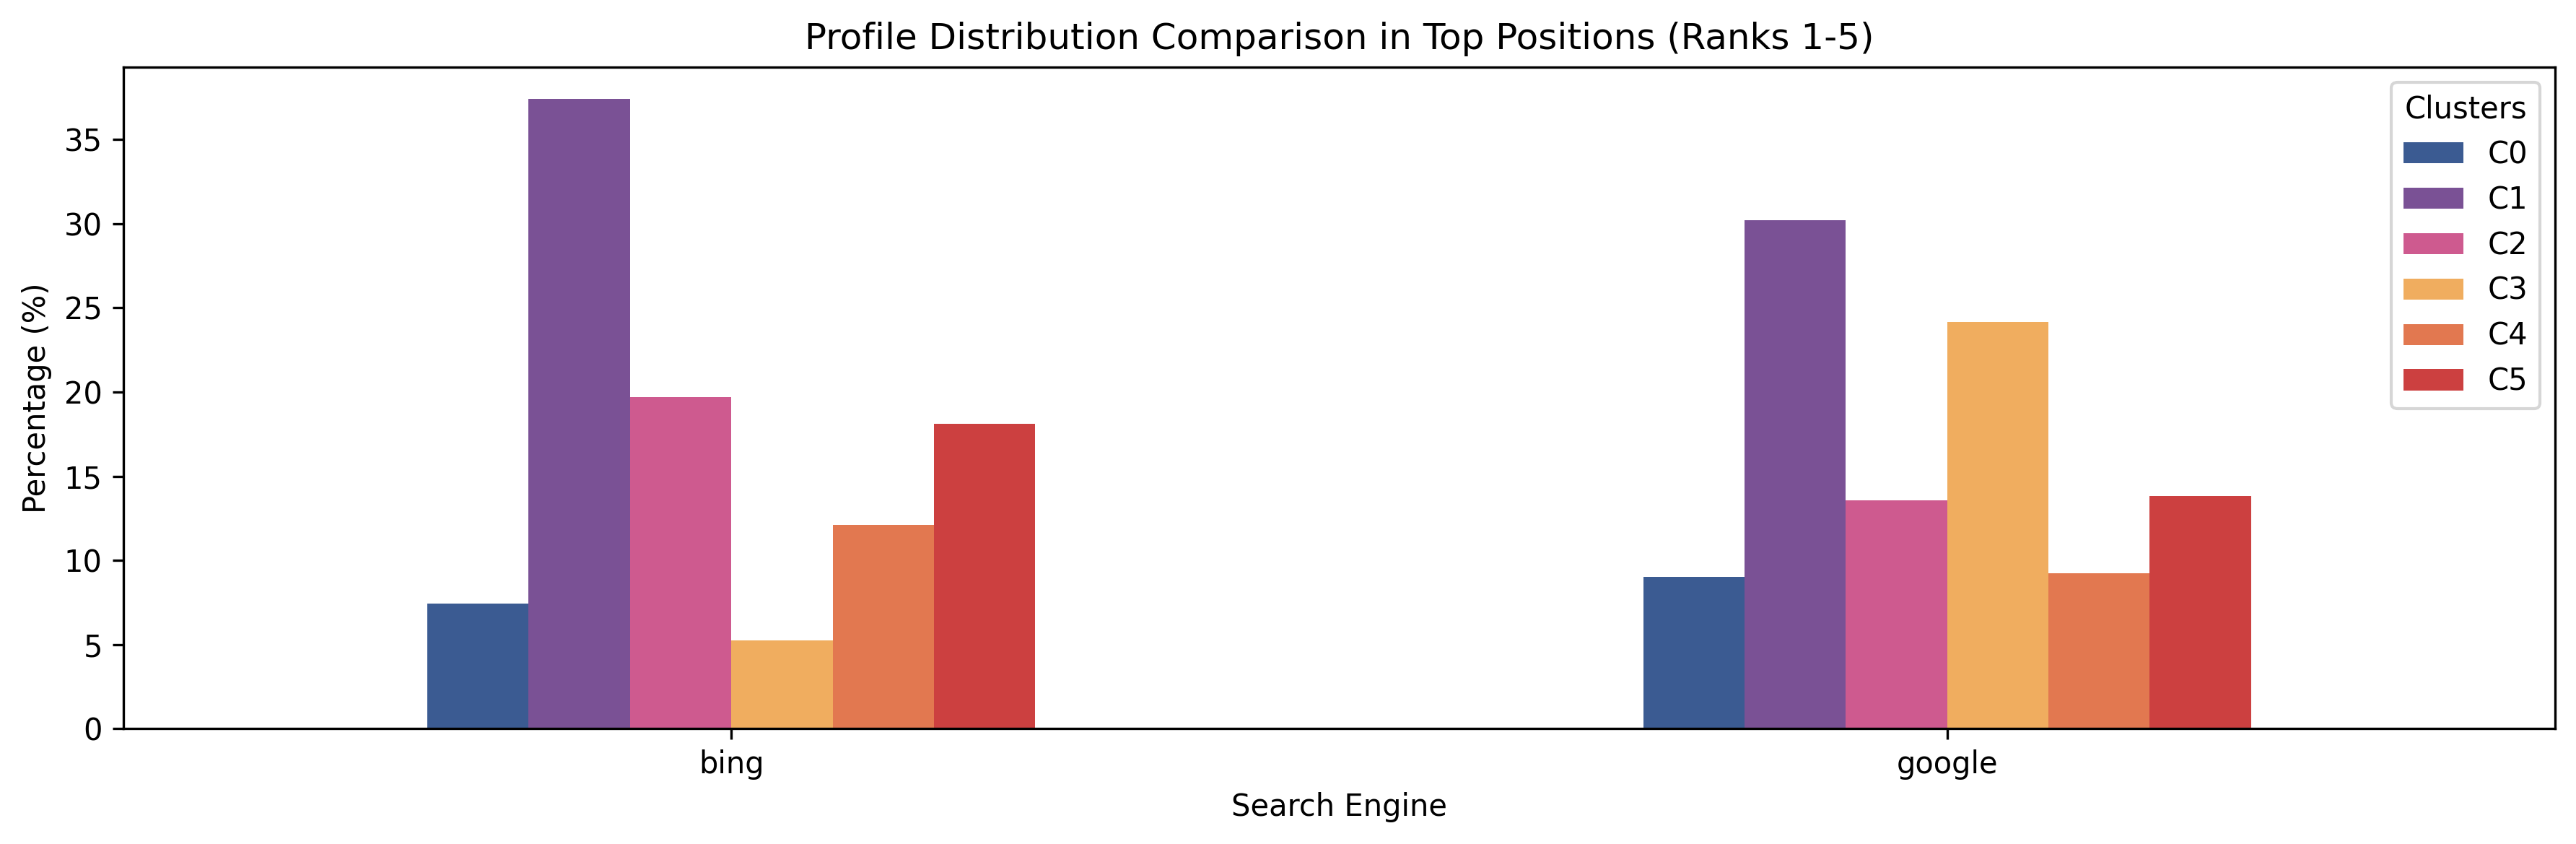
\includegraphics[width=1\linewidth]{figs/rq3_profile_comparison.png}
\caption{Comparison of Profile Distributions in Top 5 Ranks: Google vs. Bing (RQ3).}
\label{fig:rq3_profile_comparison}
\end{figure}

% Table for RQ3 Feature Comparison
\begin{table}[htbp!]
\centering
\caption{Comparison of Median Feature Values for Top-Ranking (1-5) Pages between Google and Bing (RQ3)}
\label{tab:rq3_feature_comparison}
\small 
\setlength{\tabcolsep}{3pt}
\renewcommand{\arraystretch}{1}
\begin{threeparttable}
\begin{tabular*}{\textwidth}{l@{\extracolsep{\fill}} S[table-format=3.1] S[table-format=3.1] S[table-format=1.3,table-comparator=true,table-space-text-post={***}] S[table-format=-1.3,table-space-text-post={***}]}
\toprule
\sbf{Feature} & {\sbf{Median Google}} & {\sbf{Median Bing}} & {\sbf{p-value}} & {\sbf{Cohen's d}} \\
\dmidrule
\multicolumn{5}{@{}l}{\sit{Lighthouse Scores (0-100)}} \\
Perf. & 90.0 & 92.0 & 0.002** & -0.198 \\
Access. & 91.0 & 91.0 & < .001*** & -0.297 \\
Best Prac. & 96.0 & 96.0 & < .001*** & 0.029 \\
SEO & 92.0 & 92.0 & < .001*** & -0.515 \\
\midrule
\multicolumn{5}{@{}l}{\sit{Content Relevance Metrics}} \\
Q-Title \tnote{a} & 0.0 & 0.0 & < .001*** & -0.270 \\
Q-H1 \tnote{a} & 0.0 & 0.0 & < .001*** & -0.179 \\
ExQ-Title \tnote{a} & 0.0 & 0.0 & < .001*** & -0.139 \\
ExQ-H1 \tnote{a} & 0.0 & 0.0 & < .001*** & -0.163 \\
Q/B Density (\%) & 0.0 & 0.0 & < .001*** & -0.185 \\
Sim. Title (0-1) & 0.8 & 0.8 & < .001*** & -0.570 \\
Sim. Content (0-1) & 0.6 & 0.7 & < .001*** & -0.365 \\
Word Count  & 567.0 & 630.0 & < .001*** & -0.302 \\
\bottomrule
\end{tabular*}
\begin{tablenotes}[flushleft]
\scriptsize
\item Mann-Whitney U test used. p-values: * $p < .05$; ** $p < .01$; *** $p < .001$.
\item Cohen's d: negligible ($|d| < 0.2$), small ($0.2 \le |d| < 0.5$), medium ($0.5 \le |d| < 0.8$).
\item[a] For binary features, medians are shown; mean percentages discussed in text.
\item Metric abbreviations are defined in Table \ref{tab:dataset_columns_types}.
\end{tablenotes}
\end{threeparttable}
\end{table}




\subsection{RQ4: Inferred Factor Priorities}
\label{subsec:results_rq4}
\textbf{Correlation Analysis:} Spearman rank correlations are detailed in Appendix \ref{app:rq4_correlation_heatmaps} (Figure \ref{fig:rq4_correlation_heatmaps_combined_appendix}).
\begin{itemize}
\item For Google, $\longvar{semantic_similarity_content_query}$ showed the strongest significant negative correlation with $position$ ($\rho = -0.221$), followed by $query\_in\_h1$ ($\rho \approx -0.19$) and $\longvar{semantic_similarity\_title\_query}$ ($\rho = -0.179$).
\item For Bing, $word\_count$ ($\rho = -0.257$) and $query\_density\_body$ ($\rho = -0.133$) were most notable. All these correlations had $p < .001$.
\end{itemize}

\textbf{Ordinal Logistic Regression:} (Full models are in \ref{app:rq4_regression_tables}).
\begin{itemize}
\item For Google (Combined Model Pseudo $R^2 = 0.023$), several predictors were significantly associated with better ranking quintiles. These included \longvar{semantic_similarity_content_query} (coeff: -0.475), $accessibility\_score$ (coeff: -0.154), $query\_in\_h1$ (coeff: -0.115), and $query\_in\_title$ (coeff: -0.079). Conversely, a higher \longvar{semantic_similarity_title\_query} (coeff: +0.168) and $seo\_score$ (coeff: +0.201) were significantly associated with worse ranking quintiles (all $p < .001$). Notably, $performance\_score$ was not a significant predictor in the combined model ($p = 0.294$).
\item For Bing (Combined Model Pseudo $R^2 = 0.031$), $word\_count$ emerged as the most powerful predictor of better ranking quintiles, with the largest significant negative coefficient (coeff: -1.165). Other factors significantly associated with better rankings included $accessibility\_score$ (coeff: -0.358), $exact\_query\_in\_h1$ (coeff: -0.103), \longvar{semantic_similarity_content_query} (coeff: -0.109), $query\_in\_title$ (coeff: -0.082), and $query\_density\_body$ (coeff: -0.042). In contrast, higher scores for $performance\_score$ (coeff: +0.059), $exact\_query\_in\_title$ (coeff: +0.056), and $query\_in\_h1$ (coeff: +0.053) were unexpectedly associated with worse ranking quintiles (all $p < .05$).
\end{itemize}

\textbf{Random Forest Feature Importance:} Content factors had higher aggregate importance than technical factors for both Google (70.1\%) and Bing (61.8\%) (Figure \ref{fig:rq4_feature_importance_combined}). $Word\_count$ and semantic similarity metrics were top individual content predictors.

\begin{figure}[htbp!]
\centering
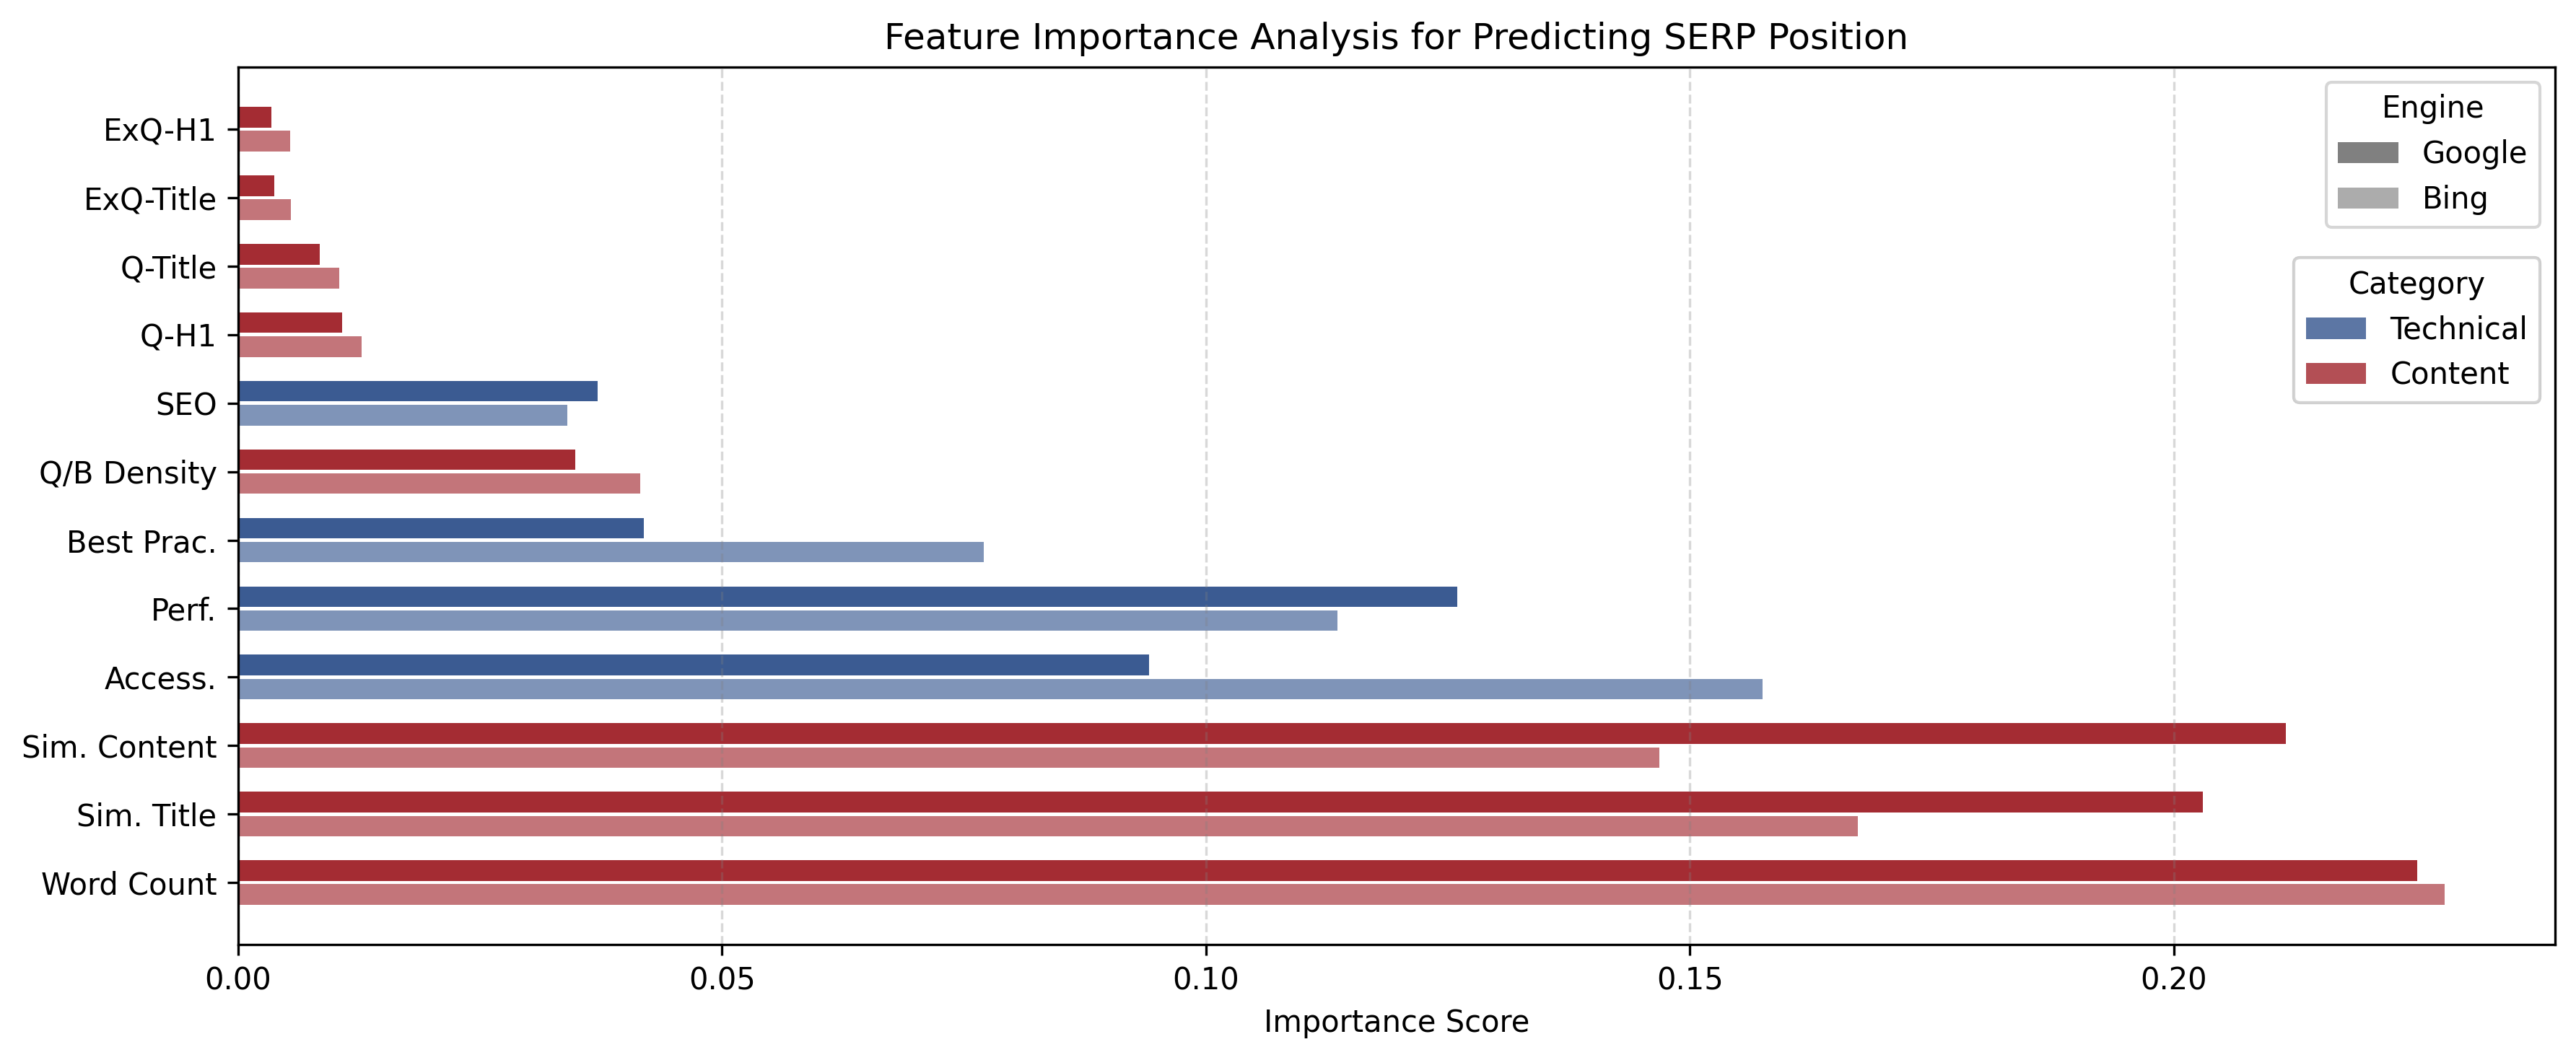
\includegraphics[width=1\linewidth]{figs/rq4_feature_importance_combined.png}
\caption{Relative feature importance from Random Forest for Google (left) and Bing (right) (RQ4).}
\label{fig:rq4_feature_importance_combined}
\end{figure}

These analyses collectively indicate that content-related attributes generally exhibit a stronger association with ranking visibility than technical scores alone. However, specific influential factors and their impact direction vary between Google and Bing and across different analytical models.
% --- END RESULTS ---


% --- DISCUSSION ---
\section{Discussion}
\label{sec:discussion}
This section interprets the empirical findings from Section \ref{sec:results}. It contextualizes them within existing literature and discusses their broader implications and limitations.

\subsection{Interpretation of Resource Profiles (RQ1)}
\label{subsec:discussion_rq1}
The K-Means clustering (RQ1) successfully delineated six distinct resource profiles within the commercial offers domain (Table \ref{tab:rq1_cluster_summary}, Figure \ref{fig:rq1_cluster_radar_normalized}). These profiles, such as "High Keyword \& Semantic Relevance, Strong Technicals" (Cluster 2) and "Low Relevance, Low Technicals" (Cluster 3), illustrate the diverse optimization strategies and quality levels present. The differentiation was significantly driven by on-page lexical features (e.g., $query\_in\_title$) and title-focused semantic similarity. This underscores their role in characterizing resources in this niche \citep{Yu2024}. This granular profiling moves beyond simplistic high/low quality categorizations, revealing a spectrum of resource archetypes.

\subsection{Inferring System Ranking Logic (RQ2 \& RQ4)}
\label{subsec:discussion_rq2_rq4}
\textbf{Profile Association with Ranking (RQ2):} For both Google and Bing, resource profiles significantly associated with ranking tiers (Figure \ref{fig:rq2_profile_dist_combined}). Stronger content-relevant profiles were generally favored in higher ranks. This aligns with the established importance of content quality \citep{Srinivas2025}.

\textbf{Individual Feature Association with Ranking (RQ2 \& RQ4):} Ordinal Logistic Regression (Appendix \ref{app:rq4_regression_tables}) and Spearman correlations (Appendix \ref{app:rq4_correlation_heatmaps}, Figure \ref{fig:rq4_correlation_heatmaps_combined_appendix}) offered deeper, and at times counter-intuitive, insights into system priorities.

For \textbf{Google}, the combined regression model underscored a complex evaluation logic. The semantic relevance of the main content (\longvar{semantic_similarity_content_query}, coeff: -0.475) and technical accessibility (\longvar{accessibility_score}, coeff: -0.154) were strong, significant predictors of a better rank. This confirms Google's focus on deep, meaningful content and foundational user-centric technicals. However, the model revealed several striking findings. The Lighthouse $performance\_score$ was not a significant predictor, suggesting that, within this competitive landscape, performance alone does not differentiate top-ranking pages once other factors are considered. Furthermore, two factors were associated with a *worse* ranking quintile: higher semantic similarity between the page title and the query (\longvar{semantic_similarity_title_query}, coeff: +0.168) and a higher Lighthouse $seo\_score$ (coeff: +0.201). These results suggest that, when other factors are controlled for, excessive or overly direct optimization targeting specific elements like titles might be perceived negatively, possibly as a signal of manipulation or low-quality optimization \citep{Nagpal2021}. Bu durum, yalnızca bir ceza mekanizması olmak yerine, daha karmaşık bir stratejinin parçası olabilir; örneğin, sistem, "sorgu belirsizliğini" (query ambiguity) yönetmek için, sorguyla mükemmel eşleşen başlıklar yerine daha geniş bağlam sunan başlıkları önceliklendirerek "sonuç çeşitliliğini" (result diversification) artırmayı hedefliyor olabilir. This approach may satisfy a broader range of user intents for a general term. Google's algorithm may favor titles that provide broader context or value beyond mere keyword matching, especially when the main content's relevance is already high.

For \textbf{Bing}, the regression analysis painted a picture of a system that, while also valuing relevance, heavily prioritizes content volume. \longvar{Word_count} emerged as the most powerful predictor of a better rank, with the largest significant negative coefficient by a substantial margin (coeff: -1.165). This implies a strong system-level preference for comprehensive, in-depth resources. Technical accessibility (\longvar{accessibility_score}, coeff: -0.358) and several explicit relevance signals like including the exact query in H1 tags (\longvar{exact_query_in_h1}, coeff: -0.103) also significantly predicted better ranks. Similar to Google, Bing's model also produced counter-intuitive results: higher scores for $performance\_score$ (coeff: +0.059) and having the exact query in the title (\longvar{exact_query_in_title}, coeff: +0.056) were unexpectedly associated with worse ranking quintiles. The negative association with performance score could be due to multicollinearity or unmeasured factors, while the title result hints that both engines may share a complex, non-linear evaluation of title optimization.

\textbf{Technical vs. Content Factors (RQ4):} Random Forest models (Figure \ref{fig:rq4_feature_importance_combined}) indicated a greater aggregate importance for content factors over technical Lighthouse scores for both Google (70.1\% content) and Bing (61.8\% content). While specific technical metrics like $accessibility\_score$ proved significant in regression, content attributes collectively showed a stronger association with visibility. This supports the "content is king" paradigm, while also affirming the non-negligible role of technical performance \citep{Roumeliotis2022}. The improved fit of combined regression models over single-factor-type models further highlights the interdependent nature of these attribute categories.

\subsection{Profiling System Differences (RQ3)}
\label{subsec:discussion_rq3}
Comparative analysis (RQ3) revealed significant operational differences between Google and Bing. Bing's top results generally featured higher median values for a majority of the measured technical and content features (Table \ref{tab:rq3_feature_comparison}), and its regression model rewarded a clear, volume-based content strategy ($word\_count$) most heavily. This suggests a more direct and perhaps more predictable ranking logic based on observable on-page factors.

In contrast, Google's logic appears more nuanced and complex. The negative coefficients for \longvar{semantic_similarity_title_query} and $seo\_score$ in its regression model, coupled with the non-significance of $performance\_score$, suggest a system that may actively discount what it interprets as overt optimization attempts. Furthermore, the higher proportion of "Low Relevance" profiles (notably Cluster 1 and Cluster 3) in Google's top results (Figure \ref{fig:rq3_profile_comparison}) could imply a greater reliance on unmeasured, off-page factors like domain authority or brand equity \citep{Toms2004}. **Bununla birlikte, bu durum kısmen veri toplama yönteminin bir sonucu da olabilir; kullanılan Google Custom Search API'sinin, canlı bir kullanıcıya sunulan son derece dinamik ve kişiselleştirilmiş sonuçlardan farklı, daha standart bir sonuç sayfası döndürme potansiyeli, veri setinde neden bazı düşük profilli sonuçların göründüğünü açıklayabilir.** This divergence suggests that Bing may currently reward a checklist-style optimization approach more reliably, whereas Google's algorithm requires a more holistic strategy that balances on-page relevance with a sophisticated, perhaps less direct, presentation.

\subsection{Synthesis and Overall Picture}
\label{subsec:discussion_synthesis}
The findings paint a picture of two distinct, though overlapping, ranking ecosystems. Visibility in both is dominated by content, but the nature of that "dominant" content differs. \textbf{Bing's logic appears to be "bigger is better,"} strongly and clearly rewarding content volume ($word\_count$, coeff: -1.165) above all else, supplemented by explicit relevance signals. \textbf{Google's logic is more enigmatic}, prioritizing the semantic depth of the main content while simultaneously showing a complex, and even punitive, response to aggressive optimization in titles (coeff: +0.168) and basic SEO metrics (coeff: +0.201). The non-significance of page speed ($performance\_score$) in Google's model is a particularly salient finding, challenging conventional SEO wisdom.

This study's most critical contribution is the unveiling of these counter-intuitive regression findings for both systems. The fact that certain "optimizations" correlate with worse rankings in a multivariate context powerfully illustrates that factors do not operate in a vacuum. A simple correlation may be misleading; the true impact of a feature is conditional on the presence and values of others. This highlights the inherent complexity of reverse-engineering modern IR systems and the pitfalls of relying on simplistic, single-factor analyses. The results strongly suggest that both algorithms have evolved beyond simple positive weighting of all "good" signals and now incorporate more sophisticated, context-dependent evaluations. Bu değerlendirmeler, yalnızca manipülatif uygulamalarla mücadele etmek için değil, aynı zamanda belirsiz sorgular için sonuç çeşitliliğini yönetmek veya uzun vadeli kullanıcı memnuniyetini öngören sinyallere öncelik vermek gibi daha gelişmiş hedeflere hizmet ediyor olabilir.

\subsection{Implications}
\label{subsec:discussion_implications}
\textbf{Practical Implications:} The updated results lead to more nuanced, actionable advice for content creators.
\begin{itemize}
\item For \textbf{Google}, the primary focus should be on creating high-quality, topically comprehensive content that is semantically rich and directly answers user intent (\longvar{semantic_similarity_content_query}). Technical accessibility must be flawless. However, creators should be wary of hyper-optimization in titles and other basic SEO elements. A title that is too semantically close to the query may be less effective than one that offers additional context or a more natural phrasing. Blindly chasing a perfect Lighthouse $seo\_score$ may be counterproductive, and while page speed ($performance\_score$) should not be ignored, it does not appear to be a deciding factor in this competitive context.
\item For \textbf{Bing}, the strategy is more straightforward: write longer, more detailed content. The strong, clear signal from the $word\_count$ coefficient suggests that content depth and volume are paramount. This should be combined with fundamental on-page practices like including exact-match keywords in H1 tags and ensuring high accessibility.
\item The existence of multiple "successful" profiles (RQ1) and the complex regression results reinforce that a one-size-fits-all approach is obsolete. Optimization must be tailored not only to the target search engine but also to the resource's intrinsic strengths.
\end{itemize}

\textbf{Theoretical Implications:} This research significantly advances the understanding of large-scale, operational "black-box" information retrieval systems, differentiating itself from prior work and contributing to IR theory in several key ways:
\begin{itemize}
\item \textbf{Unveiling Algorithmic Complexity and Non-Linearity:} This study provides robust empirical evidence that the factor weighting in major search engines is complex, non-linear, and highly context-dependent. The identification of significant negative associations for intuitively "positive" factors (e.g., \longvar{semantic_similarity_title_query} for Google; $performance\_score$ for Bing) in multivariate models challenges simplistic, additive models of ranking. It contributes to a more nuanced theoretical framework where systems may penalize perceived over-optimization or balance signals in sophisticated ways.
\item \textbf{System-Specific Ranking Philosophies:} The clear divergence between Google's complex, semantics-driven model and Bing's volume-centric approach provides strong empirical grounding for the theory that different IR systems develop distinct "ranking philosophies." This goes beyond surface-level differences and points to fundamental divergences in how relevance, quality, and user intent are modeled and operationalized.
\item \textbf{Methodology for Isolating Nuanced Signals:} By using a content-homogeneous dataset and combining multiple analytical techniques (clustering, correlation, regression, feature importance), this study presents a powerful methodology for moving beyond broad-stroke observations to uncover subtle, system-specific factor interactions. This framework provides a template for future research aiming to "reverse-engineer" opaque systems.
\item \textbf{Public Dataset for Reproducibility and Further Study:} The commitment to release the dataset and analysis scripts provides a valuable asset to the IR community, enabling replication, extension, and further exploration of these complex ranking dynamics, thereby fostering greater transparency and cumulative knowledge.
\end{itemize}

\subsection{Limitations}
\label{subsec:discussion_limitations}
This study's findings should be considered within its limitations:
\begin{itemize}
\item \textbf{Data Snapshot and Domain Specificity:} Data are from May 2025 for 500 English commercial discount queries and may not generalize.
\item \textbf{Feature Scope:} Excluded factors include backlinks, detailed Core Web Vitals, user engagement, and domain-level authority signals. Observed anomalies might be partially explained by these unmeasured variables.
\item \textbf{Tool and API Limitations:} Accuracy depends on tools like Trafilatura, Sentence-BERT, and APIs.
\item \textbf{Causation vs. Correlation:} The study identifies associations, not causal links. Inferred priorities are based on observed patterns. Actual causal mechanisms are opaque and might be influenced by unmeasured confounders or complex feature interactions not explicitly modeled.
\item \textbf{Interaction Effects:} Regression models did not explicitly include interaction terms. These could explain some complex patterns (e.g., title similarity's effect varying with content similarity). Future work should explore these.
\item \textbf{Search Engine Intent Interpretation:} Engines might interpret user intent for similar queries differently, influencing attribute prioritization. This was not directly modeled.
\item \textbf{Personalization and Localization:} Efforts to minimize these using default API settings might not entirely eliminate their influence.
\item \textbf{Scope of Baseline Comparison:} This study focused on characterizing existing search engine behaviors rather than proposing and evaluating a new ranking algorithm against state-of-the-art (SOTA) baselines. While Sentence-BERT (an LLM) was used for feature extraction, a direct comparison with LLM-based ranking models was beyond the current scope, which aimed to understand how incumbent systems respond to a defined set of features.
\end{itemize}
These limitations offer avenues for future research.
% --- END DISCUSSION ---




% --- DATA AND CODE AVAILABILITY ---
\section{Data and Code Availability}
\label{sec:data_code_availability}
The dataset generated and analyzed during the current study will be made publicly available upon acceptance of this manuscript. This includes the list of queries, raw SERP data, extracted features, and cluster labels. Similarly, the Python scripts used for data collection, feature engineering, and analysis ("SERP Profiler Kit") will also be openly shared at that time. This aims to ensure reproducibility and facilitate further research by the community. Specific repository links will be provided in the final published version.

% --- CONCLUSION ---
\section{Conclusion and Future Work}
\label{sec:conclusion}
This study empirically characterized and compared the ranking environments of Google and Bing for commercial discount queries, based on an analysis of technical and content attributes from a large number of SERP entries. Six distinct resource profiles were identified, revealing varied optimization strategies. Content-related attributes, particularly semantic relevance and (for Bing) content volume, showed a stronger overall association with ranking visibility than technical Lighthouse scores for both search engines. However, specific influential factors and their impact direction varied significantly between Google and Bing and across different analytical models.

\subsection{Principal Findings}
\label{subsec:conclusion_summary}
Key findings include:
\begin{itemize}
\item \textbf{RQ1:} Six resource profiles emerged, differentiated primarily by query presence in titles/H1s and title-query semantic similarity.
\item \textbf{RQ2:} Resource profiles significantly associated with ranking tiers in both Google and Bing. Stronger content-relevant profiles were generally more prevalent in higher ranks.
\item \textbf{RQ3:} Bing's top-ranking pages generally exhibited higher median scores for most technical and content features compared to Google's. Profile distributions in top ranks also differed significantly.
\item \textbf{RQ4:} Content factors held greater aggregate importance than technical scores for both systems. Multivariate regression revealed distinct and complex priorities: For \textbf{Google}, strong predictors of better rank included main content semantic similarity and accessibility, while high title-query semantic similarity and a high SEO score were surprisingly associated with worse rank. For \textbf{Bing}, content volume ($word\_count$) was the most powerful predictor of better rank, while factors like performance score were unexpectedly associated with worse rank.
\end{itemize}

\subsection{Concluding Remarks}
\label{subsec:conclusion_remarks}
This empirical study provides a data-driven characterization of two distinct search engine ranking philosophies. Visibility is not a simple sum of positive factors; it is shaped by a complex interplay of technical and content attributes, evaluated through different lenses by Google and Bing. The nuanced, and particularly the counter-intuitive, regression findings underscore the sophistication of modern IR algorithms and the folly of a one-size-fits-all optimization strategy. Google's logic appears to reward deep semantic relevance while penalizing overt optimization in specific elements like titles. Bing's logic seems more direct, placing a heavy premium on content volume as a proxy for authority and depth. These differing sensitivities emphasize the need for system-specific optimization strategies. We stress that these findings reveal correlations within a complex system, not simple causation. Inferred priorities should be interpreted as empirical patterns that reveal the distinct character of each search engine, not as immutable algorithmic rules.

\subsection{Future Research Directions}
\label{subsec:conclusion_future}
Future work could include: longitudinal analysis to track algorithmic changes; expanding the feature set (e.g., backlinks, Core Web Vitals, user engagement signals); applying the methodology to diverse domains and languages. Further avenues are employing advanced predictive modeling, including the exploration of interaction effects between features, or causal inference techniques. Qualitative case studies could deepen understanding of specific ranking outcomes. Finally, further investigation into anomalous findings is warranted, particularly the role of title-query semantic similarity and SEO scores in Google's regression models and performance scores in Bing's.
% --- END CONCLUSION ---

% --- ADD THE DECLARATION HERE ---
\section*{Declaration of Generative AI and AI-assisted Technologies in the Writing Process}
During the preparation of this work the author(s) used ChatGPT (OpenAI) and Gemini (Google) in order to improve language, clarity, and assist with structuring the manuscript. After using these tool\/services, the author(s) reviewed and edited the content as needed and take(s) full responsibility for the content of the published article.
% --- END OF DECLARATION ---

% --- APPENDICES ---
\clearpage
\appendix
\section{Detailed Statistical Test Results}
\label{app:detailed_stats} 
\subsection{RQ4 - Ordinal Logistic Regression Results}
\label{app:rq4_regression_tables}


% For Google
\begin{table}[htbp!] 
\centering
\caption{Ordinal Logistic Regression for Predicting SERP Quintiles - Google (System A) (RQ4)}
\label{app:rq4_regression_google}
\small 
\setlength{\tabcolsep}{3pt}
\renewcommand{\arraystretch}{1}
\begin{threeparttable}
\begin{tabular*}{\textwidth}{l@{\extracolsep{\fill}} S[table-format=-1.3,table-space-text-post={***}] S[table-format=1.3,table-comparator=true,table-space-text-post={***}] S[table-format=-1.3,table-space-text-post={***}] S[table-format=1.3,table-comparator=true,table-space-text-post={***}] S[table-format=-1.3,table-space-text-post={***}] S[table-format=1.3,table-comparator=true,table-space-text-post={***}]}
\toprule
& \multicolumn{2}{c}{\sbf{Technical Model}} & \multicolumn{2}{c}{\sbf{Content Model}} & \multicolumn{2}{c}{\sbf{Combined Model}} \\
\cmidrule(lr){2-3} \cmidrule(lr){4-5} \cmidrule(lr){6-7}
\sbf{Predictor} & {\sbf{Coeff.}} & {\sbf{p-value}} & {\sbf{Coeff.}} & {\sbf{p-value}} & {\sbf{Coeff.}} & {\sbf{p-value}} \\
\dmidrule
\sit{Lighthouse Scores} & & & & & & \\
Perf. & -0.064 & 0.016* & \multicolumn{1}{c}{--} & \multicolumn{1}{c}{--} & 0.029 & 0.294 \\
Access. & -0.208 & < .001*** & \multicolumn{1}{c}{--} & \multicolumn{1}{c}{--} & -0.154 & < .001*** \\
Best Prac. & -0.018 & 0.490 & \multicolumn{1}{c}{--} & \multicolumn{1}{c}{--} & -0.001 & 0.957 \\
SEO & 0.168 & < .001*** & \multicolumn{1}{c}{--} & \multicolumn{1}{c}{--} & 0.201 & < .001*** \\
\midrule
\sit{Content Metrics} & & & & & & \\
Q-Title & \multicolumn{1}{c}{--} & \multicolumn{1}{c}{--} & -0.070 & 0.041* & -0.079 & 0.021* \\
Q-H1 & \multicolumn{1}{c}{--} & \multicolumn{1}{c}{--} & -0.121 & < .001*** & -0.115 & < .001*** \\
ExQ-Title & \multicolumn{1}{c}{--} & \multicolumn{1}{c}{--} & -0.044 & 0.238 & -0.032 & 0.392 \\
ExQ-H1 & \multicolumn{1}{c}{--} & \multicolumn{1}{c}{--} & 0.005 & 0.896 & 0.011 & 0.764 \\
Q/B Density & \multicolumn{1}{c}{--} & \multicolumn{1}{c}{--} & 0.040 & 0.122 & 0.009 & 0.726 \\
Sim. Title & \multicolumn{1}{c}{--} & \multicolumn{1}{c}{--} & 0.202 & < .001*** & 0.168 & < .001*** \\
Sim. Content & \multicolumn{1}{c}{--} & \multicolumn{1}{c}{--} & -0.485 & < .001*** & -0.475 & < .001*** \\
Word Count & \multicolumn{1}{c}{--} & \multicolumn{1}{c}{--} & 0.045 & 0.055 & 0.033 & 0.156 \\
\midrule
Pseudo $R^2$ & \multicolumn{2}{c}{0.0046} & \multicolumn{2}{c}{0.0194} & \multicolumn{2}{c}{0.0233} \\
AIC & \multicolumn{2}{c}{18750.1} & \multicolumn{2}{c}{18480.5} & \multicolumn{2}{c}{18415.5} \\
BIC & \multicolumn{2}{c}{18522.5} & \multicolumn{2}{c}{18560.7} & \multicolumn{2}{c}{18522.5} \\
\bottomrule
\end{tabular*}
\begin{tablenotes}[flushleft]
\scriptsize
\item Dependent Variable: SERP Quintile (0=best, 4=worst). Negative coefficients indicate increased likelihood of better ranking.
\item * $p < .05$; ** $p < .01$; *** $p < .001$. Thresholds (cut-points) for quintiles are omitted. Predictors Min-Max scaled.
\item Metric abbreviations are defined in Table \ref{tab:dataset_columns_types}.
\end{tablenotes}
\end{threeparttable}
\end{table}



% For Bing
\begin{table}[htbp!] 
\centering
\caption{Ordinal Logistic Regression for Predicting SERP Quintiles - Bing (System B) (RQ4)}
\label{app:rq4_regression_bing}
\small 
\setlength{\tabcolsep}{3pt}
\renewcommand{\arraystretch}{1}
\begin{threeparttable}
\begin{tabular*}{\textwidth}{l@{\extracolsep{\fill}} S[table-format=-1.3,table-space-text-post={***}] S[table-format=1.3,table-comparator=true,table-space-text-post={***}] S[table-format=-1.3,table-space-text-post={***}] S[table-format=1.3,table-comparator=true,table-space-text-post={***}] S[table-format=-1.3,table-space-text-post={***}] S[table-format=1.3,table-comparator=true,table-space-text-post={***}]}
\toprule
& \multicolumn{2}{c}{\sbf{Technical Model}} & \multicolumn{2}{c}{\sbf{Content Model}} & \multicolumn{2}{c}{\sbf{Combined Model}} \\
\cmidrule(lr){2-3} \cmidrule(lr){4-5} \cmidrule(lr){6-7}
\sbf{Predictor} & {\sbf{Coeff.}} & {\sbf{p-value}} & {\sbf{Coeff.}} & {\sbf{p-value}} & {\sbf{Coeff.}} & {\sbf{p-value}} \\
\dmidrule
\sit{Lighthouse Scores} & & & & & & \\
Perf. & 0.093 & < .001*** & \multicolumn{1}{c}{--} & \multicolumn{1}{c}{--} & 0.059 & 0.005** \\
Access. & -0.339 & < .001*** & \multicolumn{1}{c}{--} & \multicolumn{1}{c}{--} & -0.358 & < .001*** \\
Best Prac. & 0.026 & 0.223 & \multicolumn{1}{c}{--} & \multicolumn{1}{c}{--} & 0.017 & 0.415 \\
SEO & -0.080 & < .001*** & \multicolumn{1}{c}{--} & \multicolumn{1}{c}{--} & -0.029 & 0.180 \\
\midrule
\sit{Content Metrics} & & & & & & \\
Q-Title & \multicolumn{1}{c}{--} & \multicolumn{1}{c}{--} & -0.078 & 0.003** & -0.082 & 0.002** \\
Q-H1 & \multicolumn{1}{c}{--} & \multicolumn{1}{c}{--} & 0.022 & 0.394 & 0.053 & 0.043* \\
ExQ-Title & \multicolumn{1}{c}{--} & \multicolumn{1}{c}{--} & 0.064 & 0.024* & 0.056 & 0.047* \\
ExQ-H1 & \multicolumn{1}{c}{--} & \multicolumn{1}{c}{--} & -0.085 & 0.003** & -0.103 & < .001*** \\
Q/B Density & \multicolumn{1}{c}{--} & \multicolumn{1}{c}{--} & -0.036 & 0.079 & -0.042 & 0.038* \\
Sim. Title & \multicolumn{1}{c}{--} & \multicolumn{1}{c}{--} & -0.066 & 0.010** & -0.011 & 0.686 \\
Sim. Content & \multicolumn{1}{c}{--} & \multicolumn{1}{c}{--} & -0.093 & < .001*** & -0.109 & < .001*** \\
Word Count & \multicolumn{1}{c}{--} & \multicolumn{1}{c}{--} & -1.133 & < .001*** & -1.165 & < .001*** \\
\midrule
Pseudo $R^2$ & \multicolumn{2}{c}{0.0131} & \multicolumn{2}{c}{0.0188} & \multicolumn{2}{c}{0.0310} \\
AIC & \multicolumn{2}{c}{27222.5} & \multicolumn{2}{c}{27074.1} & \multicolumn{2}{c}{26745.8} \\
BIC & \multicolumn{2}{c}{26858.7} & \multicolumn{2}{c}{27158.8} & \multicolumn{2}{c}{26858.7} \\
\bottomrule
\end{tabular*}
\begin{tablenotes}[flushleft]
\scriptsize
\item Dependent Variable: SERP Quintile (0=best, 4=worst). Negative coefficients indicate increased likelihood of better ranking.
\item * $p < .05$; ** $p < .01$; *** $p < .001$. Thresholds (cut-points) for quintiles are omitted. Predictors Min-Max scaled.
\item Metric abbreviations are defined in Table \ref{tab:dataset_columns_types}.
\end{tablenotes}
\end{threeparttable}
\end{table}




\afterpage{
\begin{sidewaysfigure}
\centering
\subsection{RQ4 - Spearman Correlation Heatmaps}
\label{app:rq4_correlation_heatmaps}
% \vspace*{-2cm}
% \hspace*{-4.5cm}
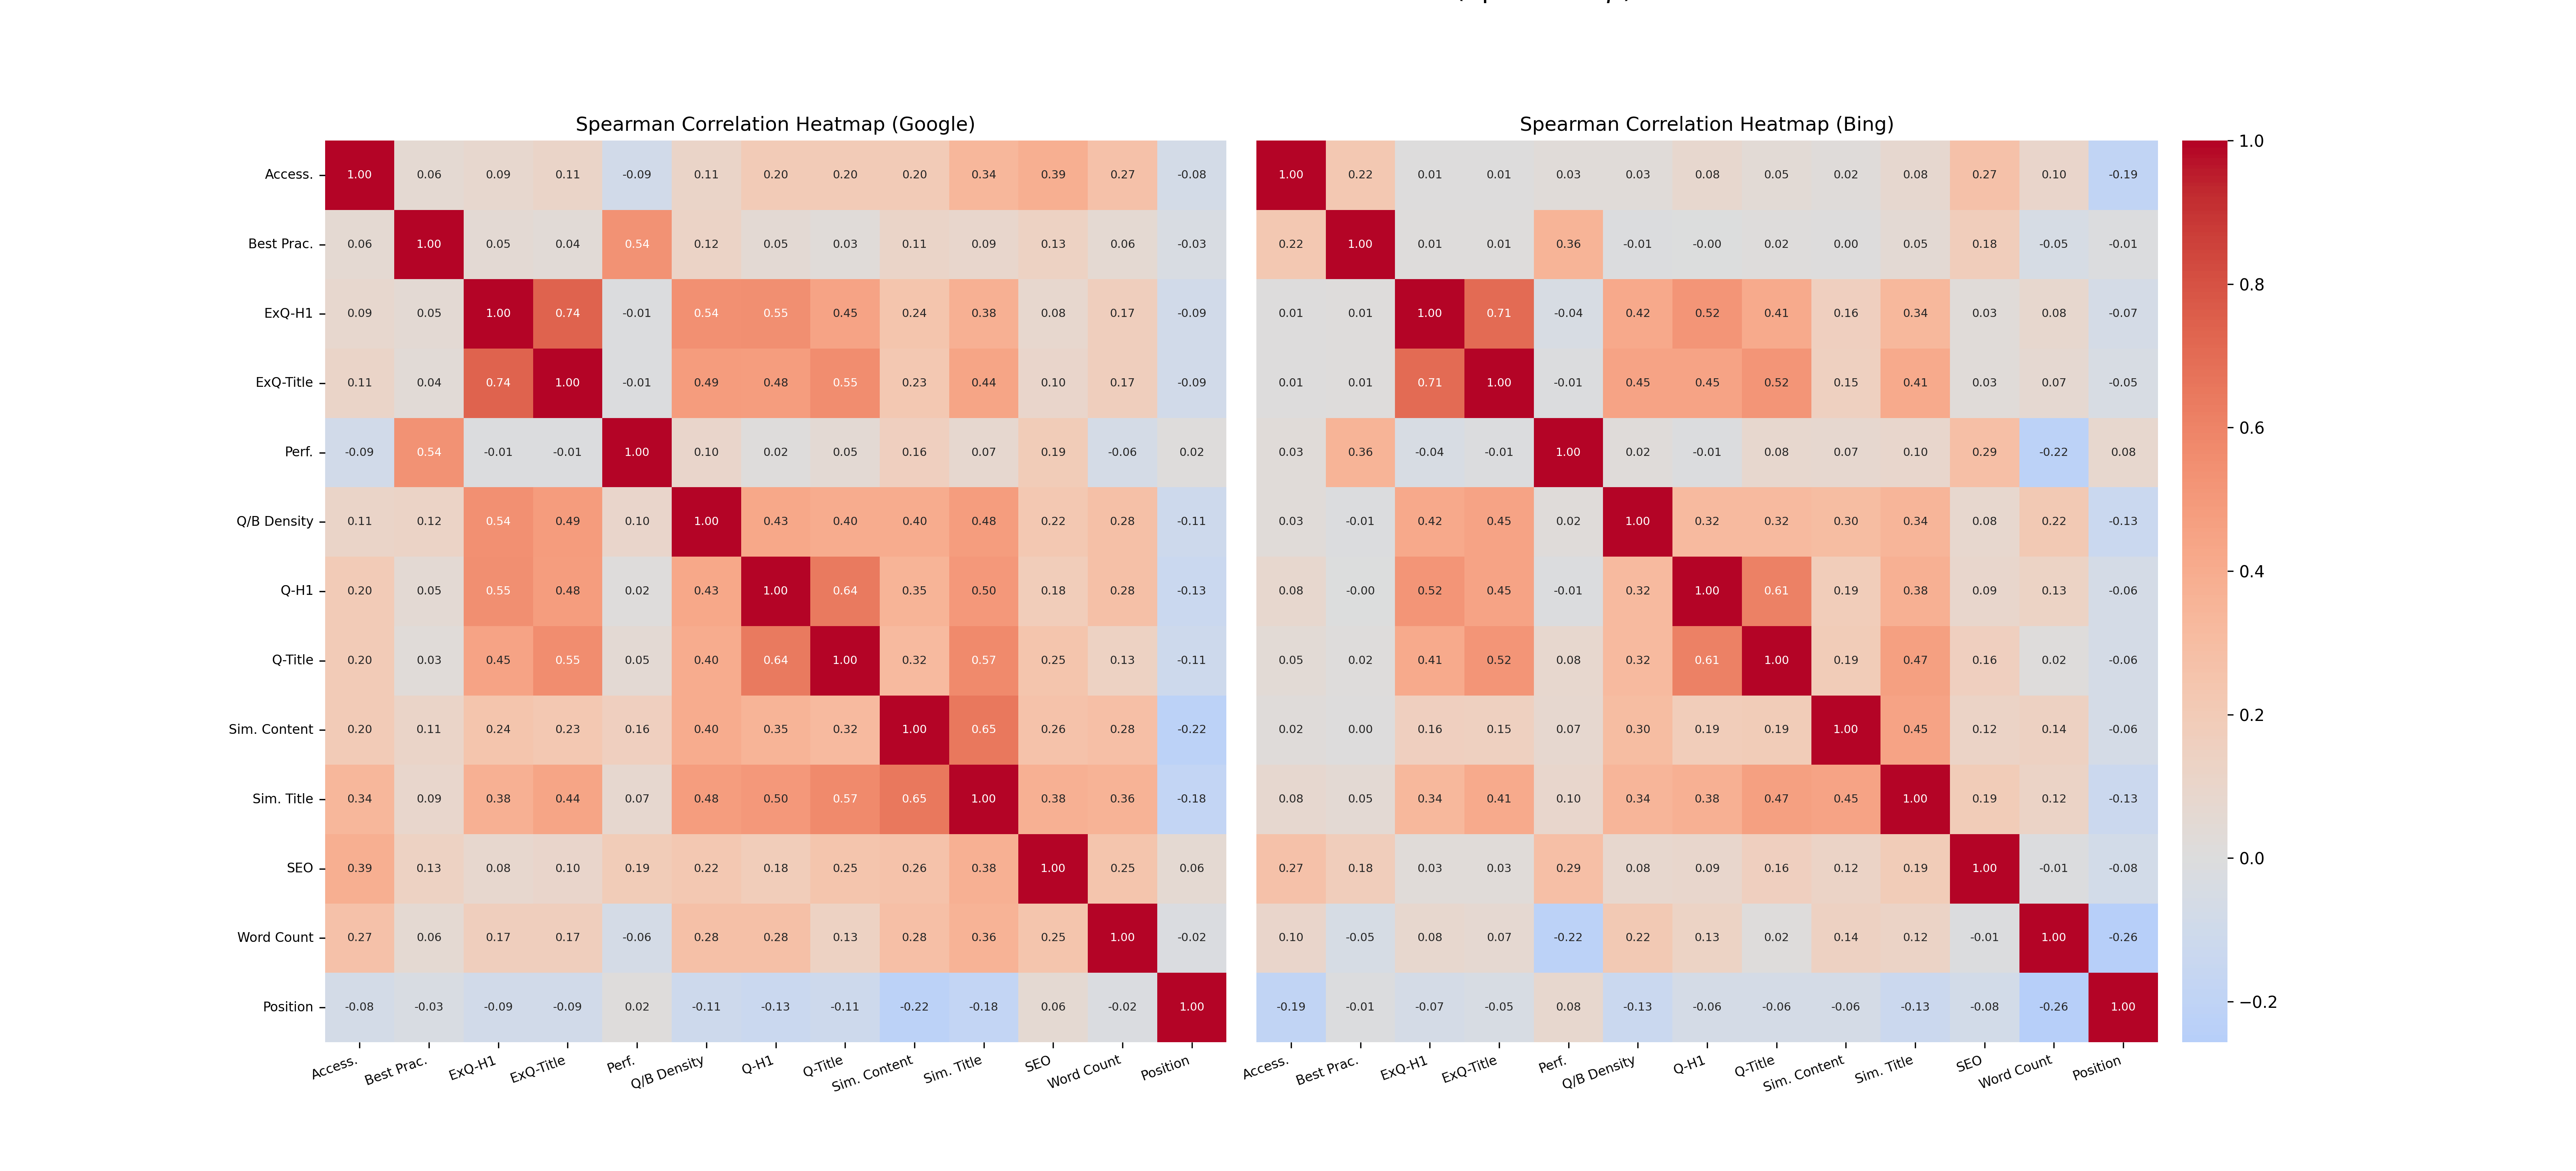
\includegraphics[width=1.1\textwidth,trim={2cm 0 2cm 0},clip]{figs/rq4_correlation_heatmaps_combined.png}
\caption{Spearman Correlation Heatmaps with SERP Position for Google (left) and Bing (right) (RQ4).}
\label{fig:rq4_correlation_heatmaps_combined_appendix}
\end{sidewaysfigure}
}


% \section{My Appendix}
% Appendix sections are coded under \verb+\appendix+.

% \verb+\printcredits+ command is used after appendix sections to list 
% author credit taxonomy contribution roles tagged using \verb+\credit+ 
% in frontmatter.

\printcredits

\FloatBarrier
\clearpage
%% Loading bibliography style file
% \bibliographystyle{model1-num-names}
\bibliographystyle{cas-model2-names}

% Loading bibliography database
\bibliography{cas-refs}


%\vskip3pt

% \bio{figs/pic1}
% Author biography with author photo.
% Author biography. Author biography. Author biography.
% Author biography. Author biography. Author biography.
% Author biography. Author biography. Author biography.
% Author biography. Author biography. Author biography.
% Author biography. Author biography. Author biography.
% Author biography. Author biography. Author biography.
% Author biography. Author biography. Author biography.
% Author biography. Author biography. Author biography.
% Author biography. Author biography. Author biography.
% \endbio

% \bio{figs/pic1}
% Author biography with author photo.
% Author biography. Author biography. Author biography.
% Author biography. Author biography. Author biography.
% Author biography. Author biography. Author biography.
% Author biography. Author biography. Author biography.
% \endbio

\end{document}
